\documentclass{sig-alternate-05-2015}

\makeatletter
\setcounter{tocdepth}{3}
\def\contentsname{Contents}
\def\tableofcontents{%
    \section*{\MakeUppercase{\contentsname}}%
    \@starttoc{toc}%
    }
\makeatother

\newcommand{\TITLE}{Cloud Metrics for Academic Resource Providers}

\newcommand{\AUTHOR}{ Gregor von Laszewski, Hyungro Lee, Fugang Wang} 

%%%%%%%%%%%%%%%%%%%%%%%%%%%%%%%%%%%%%%%%%%%%%%%%%%%%%%%%%%%%%%

% LATEX DEFINITIONS 
%%%%%%%%%%%%%%%%%%%%%%%%%%%%%%%%%%%%%%%%%%%%%%%%%%%%%%%%%%%%%%

\usepackage[colorlinks]{hyperref}
\usepackage{array} 
\usepackage{graphicx} 
\usepackage{booktabs} 
\usepackage{pifont} 
\usepackage[colorinlistoftodos]{todonotes}
\usepackage{rotating} 
\usepackage{color} 
\usepackage{listings}
\usepackage{enumitem}
\usepackage{fancyvrb}
%\usepackage{titling}



\newcommand*\rot{\rotatebox{90}} 
 
%\newcommand{\FILE}[1]{\todo[color=green!40]{#1}} 


\newcommand{\hyungro}[1]{\todo[inline, color=green!20]{Hyungro:~#1}} 
\newcommand{\gregor}[1]{\todo[inline, color=blue!20]{Gregor:~#1}} 
\newcommand{\task}[1]{\smallskip\todo[inline, color=gray!20]{#1}} 
\newcommand{\improve}[1]{\smallskip\todo[inline, color=gray!20]{old: #1}} 

%\setlist[itemize]{noitemsep, topsep=0pt} 
%%%%%%%%%%%%%%%%%%%%%%%%%%%%%%%%%%%%%%%%%%%%%%%%%%%%%%%%%%%%%%
% HYPERSETUP 
%%%%%%%%%%%%%%%%%%%%%%%%%%%%%%%%%%%%%%%%%%%%%%%%%%%%%%%%%%%%%%

\hypersetup{ 
    bookmarks=true,         % show bookmarks bar 
    unicode=false,          % non-Latin characters in Acrobat’s bookmarks 
    pdftoolbar=true,        % show Acrobat’s toolbar 
    pdfmenubar=true,        % show Acrobat’s menu 
    pdffitwindow=false,     % window fit to page when opened 
    pdfstartview={FitH},    % fits the width of the page to the window 
    pdftitle={\TITLE},    % title 
    pdfauthor={\AUTHOR},     % author 
    pdfsubject={Subject},   % subject of the document 
    pdfcreator={Gregor von Laszewski, Fugang Wang},   % creator of the document 
    pdfproducer={Gregor von Laszewski}, % producer of the document 
    pdfkeywords={hindex} {metric}{FutureGrid}, % list of keywords 
    pdfnewwindow=true,      % links in new window 
    colorlinks=false,       % false: boxed links; true: colored links 
    linkcolor=red,          % color of internal links (change box color with linkbordercolor) 
    citecolor=green,        % color of links to bibliography 
    filecolor=magenta,      % color of file links 
    urlcolor=cyan           % color of external links 
} 
 
%%%%%%%%%%%%%%%%%%%%%%%%%%%%%%%%%%%%%%%%%%%%%%%%%%%%%%%%%%%%%%%%%%%%%% 



\lstset{frame=tb,
language=sh,
aboveskip=3mm,
belowskip=3mm,
showstringspaces=false,
columns=flexible,
basicstyle={\scriptsize\ttfamily},
numbers=none,
numberstyle=\tiny\color{gray},
keywordstyle=\color{blue},
commentstyle=\color{dkgreen},
stringstyle=\color{mauve},
breaklines=true,
breakatwhitespace=true
tabsize=3
}
\begin{document} 
% 
% --- Author Metadata here --- 
\conferenceinfo{Report}{Permission to make digital or hard copies of all or part of this work for personal or classroom use is granted without fee provided that copies are not made or distributed for profit or commercial advantage and that copies bear this notice and the full citation on the first page. To copy otherwise, or republish, to post on servers or to redistribute to lists, requires prior specific permission and/or a fee.
%SAC’10, March 22-26, 2010, Sierre, Switzerland.
%Copyright 2010 ACM 978-1-60558-638-0/10/03…\$10.00.
}
\CopyrightYear{2015}  
\crdata{X-XXXXX-XX-X/XX/XX}  % Allows default copyright data (0-89791-88-6/97/05) to be over-ridden - IF NEED BE. 
% --- End of Author Metadata --- 
 
\title{\TITLE} 
%\subtitle{[Extended Abstract] 
%\titlenote{A full version of this paper is available as 
%\texttt{www.acm.org/eaddress.htm}}} 
 
\numberofauthors{1}

\author{ 
\alignauthor
Gregor  von Laszewski $^1$\titlenote{Corresponding Author.}, Hyungro Lee$^1$, Fugang Wang$^1$, Geoffrey C. Fox$^1$, \\
Thomas Furlani$^2$, Robert DeLeon$^2$, Qiao Chunming$^2$\\
       \smallskip
       \affaddr{$^1$Indiana University, 2719 10th Street, Bloomington, Indiana, U.S.A.}\\ 
       \affaddr{$^2$SUNY at Buffalo, 701 Ellicott Street, Buffalo, New York, 14203, U.S.A.}\\ 
       \smallskip\email{$^*$laszewski@gmail.com} 
}
\date{24 March 2014}  

\newpage 
{\flushleft\bf \TITLE}
\tableofcontents

\newpage
\listoftodos[Notes]
\newpage
\toappear{} 
\maketitle 
\begin{abstract} 

  Cloud computing has established itself as one of the key components
  in modern datacenters. This includes academic, government, and for
  profit institutions and organizations. One of the important aspects
  to a successfully operational cloud is the availability of
  sophisticated metric information and frameworks to assure a number
  of key operational factors. We provide an overview of the different
  aspects that are shaping the need for cloud metrics.  We especially
  identify the needs for cloud metrics and monitoring solutions for
  various user communities that are an important aspect for cloud
  providers. The motivation for cloud metrics are shaped by
  application users, administrators, service providers and funders.
  Metrics include usage, failure and auditing data to identify user
  and system behavior. Many of the metrics presented here have been
  used as part of the FutureGrid and FutureSystems clouds. This
  includes also the unified metrics service framework allowing
  integration of metrics from heterogeneous clouds such as OpenStack,
  Eucalyptus and Nimbus. Additionally, we see the importance of
  metrics also in higher level platform as a services delivered
  through the various user communities. Thus it is important to
  identify common features of existing and future services that
  benefit from metrics and their exposure to its users.



  \begin{comment} 

    In shared resource environments, usage data is necessary to
    identify utilization of the infrastructure by users. Many cloud
    platforms recently started to collect measurements for use of
    resources that can be applied to billing and
    monitoring. Understanding utilization and performance through
    these measurements is crucial in the infrastructure in order to
    provide better cloud provisioning, system management and capacity
    planning. In this paper, we present an integrated cloud accounting
    solution applicable to federated cloud environments. We have
    tested this framework on FutureGrid.  Our system is integrated as
    a CloudMetric component into a larger framework called cloudmesh
    that targets explicit user or administor controlled federation of
    clouds.  Our cloudmesh CloudMetrics component is ablehich is an
    XSEDE resources. Based on the observation on FutureGrid, we found
    that different patterns between scientific research projects and
    educational projects regarding the type of virtual machines (VMs)
    and the patterns of using virtual resources.  CloudMetrics enables
    users and project leaders to identify utilization and performance.

\end{comment}

\end{abstract} 

% %%%%%%%%%%%%%%%%%%%%%%%%%%%%%%%%%%%%%%%%%%%%%%%%%%%%%%%%%%%%%%%%%%%%%%
% ACM CLASSIFICATION, Terms, Keywords,
% %%%%%%%%%%%%%%%%%%%%%%%%%%%%%%%%%%%%%%%%%%%%%%%%%%%%%%%%%%%%%%%%%%%%%%
\begin{CCSXML}
<ccs2012>
<concept>
<concept_id>10002944.10011123.10011124</concept_id>
<concept_desc>General and reference~Metrics</concept_desc>
<concept_significance>500</concept_significance>
</concept>
<concept>
<concept_id>10003033.10003099.10003100</concept_id>
<concept_desc>Networks~Cloud computing</concept_desc>
<concept_significance>500</concept_significance>
</concept>
</ccs2012>
\end{CCSXML}

\ccsdesc[500]{Networks~Cloud computing}
\ccsdesc[500]{General and reference~Metrics}

\printccsdesc

\keywords{Cloud Metrics, Resource Monitoring, Cloud Accounting, Metering, FutureGrid, FutureSystems, XSEDE} 

%%%%%%%%%%%%%%%%%%%%%%%%%%%%%%%%%%%%%%%%%%%%%%%%%%%%%%%%%%%%%%%%%%%%%% 
% SECTIONS 
%%%%%%%%%%%%%%%%%%%%%%%%%%%%%%%%%%%%%%%%%%%%%%%%%%%%%%%%%%%%%%%%%%%%%% 

\begin{comment}
\section{OLD ABSTRACT} 


In shared resource environments, usage data is necessary to identify
utilization of the infrastructure by users. Many cloud platforms recently
started to collect measurements for use of resources that can be applied to
billing and monitoring. Understanding utilization and performance through these
measurements is crucial in the infrastructure in order to provide better cloud
provisioning, system management and capacity planning. In this paper, we
present an integrated cloud accounting solution, Cloud Metrics, to measure
cloud resource usage across several cloud platforms such as OpenStack, Nimbus,
and Eucalyptus. The usage data allows a user to see as how all resources are
efficiently supplied to their applications and discover patterns from
cumulative data. With Cloud Metrics, virtual resources such as compute, storage
and network are measured to evaluate time and cost of user applications and the
statistics for these resources offer visibility to utilization of cloud
resources. This article shows statistical analysis of several case studies by
tracing resource allocation on FutureGrid. Based on the observation on
FutureGrid, we found that different patterns between scientific research
projects and educational projects regarding the type of virtual machines (VMs)
and the patterns of using virtual resources. Cloud Metrics enables users and
project leaders to identify utilization and performance.

\todo[inline]{remove old abstract, but read if there is info we need
  to maintain.}
\end{comment}

%%%%%%%%%%%%%%%%%%%%%%%%%%%%%%%%%%%%%%%%%%%%%%%%%%%%%%%%%%%%%%%%%%%%%%
\section{INTRODUCTION}
%%%%%%%%%%%%%%%%%%%%%%%%%%%%%%%%%%%%%%%%%%%%%%%%%%%%%%%%%%%%%%%%%%%%%%

\subsection{Cloud Computing}

Cloud computing has established itself as one of the key components in
modern datacenters. This includes academic, government, and for profit
institutions and organizations.  According the NIST definition ``Cloud
computing is a model for enabling ubiquitous, convenient, on-demand
network access to a shared pool of configurable computing resources
(e.g., networks, servers, storage, applications, and services) that
can be rapidly provisioned and released with minimal management effort
or service provider interaction''~\cite{mell2011nist}. Essential
characteristics include on-demand self-service, broad network access,
rapid elasticity, measured service. Important service models are
Software as a Service (SaaS), Software as a Service (SaaS), and
Infrastructure as a Service (IaaS). Deployments include typically
private clouds, community clouds, public clouds, and hybrid clouds.

\subsection{Academic Cloud Computing}

Academic cloud computing offers clouds to the academic community. In
contrast to commercial offerings they may have some very specific
properties that need to be considered. First we distinguish two
different target communities. On the one hand includes the operational
IT organization that may provide e-mail, calendars, and document
sharing environments to the staff members of the university. The
demands for them are typically not different from any other
organization running operational production services. On the other
institutions are in the need to provide infrastructures, services, and
platforms to the academic research and education community. We will
focus in this paper on the latter communities.

Within the offerings to the academic community we observe the usage of
the following clouds (a) commercial public clouds, Academic public
clouds, and Academic private clouds. Furthermore, traditional high
performance computing )HPC) is offered as a platform in many
organizations and allows to support the paradigm of {\it HPC in the
  cloud} as showcased for example by the XSEDE project (see
Section~\ref {S:resources} for more details). The validity of HPC as a
service in the cloud is reflected not only by academic offerings, but
also by commercial offerings commercial offerings as demonstrated by
Amazon High Performance Computing~\cite{awshpc}, IBM Platform
Computing~\cite{ibmhpc}, and with additional examples provided
in~\cite{DouglasEadline}.

% How Cost Efficient is HPC in the Cloud?~\cite{WolfgangGentzsch}





\subsection{Cloud Metrics}

One of the important aspects to a successfully operational cloud is
the availability of sophisticated metric information and frameworks to
assure a number of key operational factors. As cloud computing is
typically part of a large scale data center it touches and also must
integrate common data center metrics. Furthermore, it is essential to
cloud specific application metrics while benchmarking a cloud at
regular intervals to detect potential issues. Cloud metrics are
important to a number of users interested in the various aspects
dealing with a operation, use, and management of a cloud. Hence, the
motivation for cloud metrics are shaped by application users,
administrators, service providers and funders. Metrics include usage,
failure and auditing data to identify user and system behavior. Many
of the metrics presented here have been used as part of the FutureGrid
and FutureSystems clouds. These general aspects are not only common to
a particular IaaS framework but are common across heterogeneous cloud
IaaS such as OpenStack, Eucalyptus and Nimbus including unified
metrics across such deployments.  Additionally, we see the importance
of metrics also in higher level platform as a services delivered as
part of high level cloud services designed to support various user
communities and virtual organizations. Thus it is important to
identify common features of existing and future services that benefit
from metrics and their exposure to its users. Based on our short
introduction it is clear that a more formal approach is needed to
identify

\begin{enumerate}
\setlength\itemsep{-2pt}
\item Which metrics are useful for whom and why?
\item Which metric efforts exists?
\item Which community is targeted?
\item Which services are targeted?
\item Which resources are monitored?
\item What privacy aspects exist? 
\end{enumerate}

We observe that in may cases there is no distinction between academic,
or non academic resource providers. Areas where there exists
distinction are metrics based on charging models, and the utilization
of hybrid clouds. Furthermore, we find that higher level metrics and
metrics integrating into other frameworks provided as PaaS and HPC
frameworks. The reason for this is that some projects may require a
combination of technologies that motivate project wide metrics to not
only display usage and utilization of the various frameworks and
services for these projects. The pooling of resources in a
heterogeneous environment provides a {\it computational mesh} going
potentially beyond just the utilization of cloud, HPC, and Grid
computing all of which may need to be integrated into a comprehensive
metrics framework. Due to the limited resources in academic
organizations we also often do not have (when private clouds) are
utilized an unlimited resource pool. For example the XSEDE resources
receive resource requests that are four times higher than the
available resources. Hence, it is important to identify performance
metrics and benchmarks that lead to an improvement of the applications
using such resources. For academic cloud resources availability and
scalability also need to be ensured to manage rapid changes (which we
see for example in educational usage patterns as part of classes) in the
demands for cloud resources. These characteristics of cloud computing
can be satisfied with the support of performance analysis and
monitoring. There are some considerations when performance analysis
and monitoring are applied to cloud computing: (a) performance
isolation against interference (b) availability and Scalability (c)
cost effectiveness to fully utilize available resources.


As other clouds academic clouds rely on sharing of the offered
services. However, just as in public clouds many users may not
understand the implication and cost that is prevalent when using a
particular service. Hence detailed metrics informing the user not only
at time of an experiment, but access to information that helps planing
such experiments are needed. Thus metrics will address and provide an
essential input to several concrete challenges for academic clouds
including:

\begin{description}
\setlength\itemsep{-2pt}

\item[\it Understanding] - how reliable the system is and to prevent
  system failures. It also gives an opportunity to manage the system
  efficiently by knowing the performance of the system.

\item[\it Getting informed] - of the current status and the impact of
  previous activities allowing the various user communities to act
  appropriately and invoke defensive measures as well as being an
  input to btter understanding the system over time.

\item[\it Estimating future requests] - it discovers usage patterns
  and trends of system resources which allows to projection the
  increasing of system capacity and performance.

\item[\it Reporting] - Measured statistics can be viewed in different
  ways with various visualization tools. Several graphical tools and
  charts APIs can help identify which resources are consumed the most
  by whom, what, where, why and when.

\end{description}

These and other aspects are addressed in the following paper. Our
paper is structured as follows. In Section~\ref{S:factors} we
introduce some major factors that need to be considered when providing
a cloud monitoring and metric framework. We introduce some concrete
metrics in Section~\ref{S:metrics}.  A brief summary of Monitoring
tools and services is provided in Section~\ref{S:tools}.
Section~\ref{S:cloudmesh} showcases our hybrid cloud monitoring and
metrics services that have been used in FutureGrid and are currently
used in FutureSystems. Related activities are briefly summarized in
Section~\ref{S:related}.  We conclude our paper while summarizing our
findings in Section~\ref{S:conclusion}.

%%%%%%%%%%%%%%%%%%%%%%%%%%%%%%%%%%%%%%%%%%%%%%%%%%%%%%%%%%%%%%%%%%%%%%
\section{CLOUD METRIC FACTORS} \label {S:factors}
%%%%%%%%%%%%%%%%%%%%%%%%%%%%%%%%%%%%%%%%%%%%%%%%%%%%%%%%%%%%%%%%%%%%%%

When we look at a particular cloud metric, it may be shaped by a
number of factors that determines the applicability and usability of
the metric in general. To provide an overview of a selected number of
factors fro cloud metrics we have identified the following factors of
significant importance: (a) stakeholders and roles to address, (b) the
frameworks to address, (c) the purpose the metrics are designed for,
(d) concrete resources are targeted by the metric, (e) which sources
are used for the metric, and (f) which security aspects are
considered. We are summarizing these influential aspects in Figure
\ref{F:taxonomy-1} and explaining them in more detail.

\begin{figure}[h!] 
  \centering 
    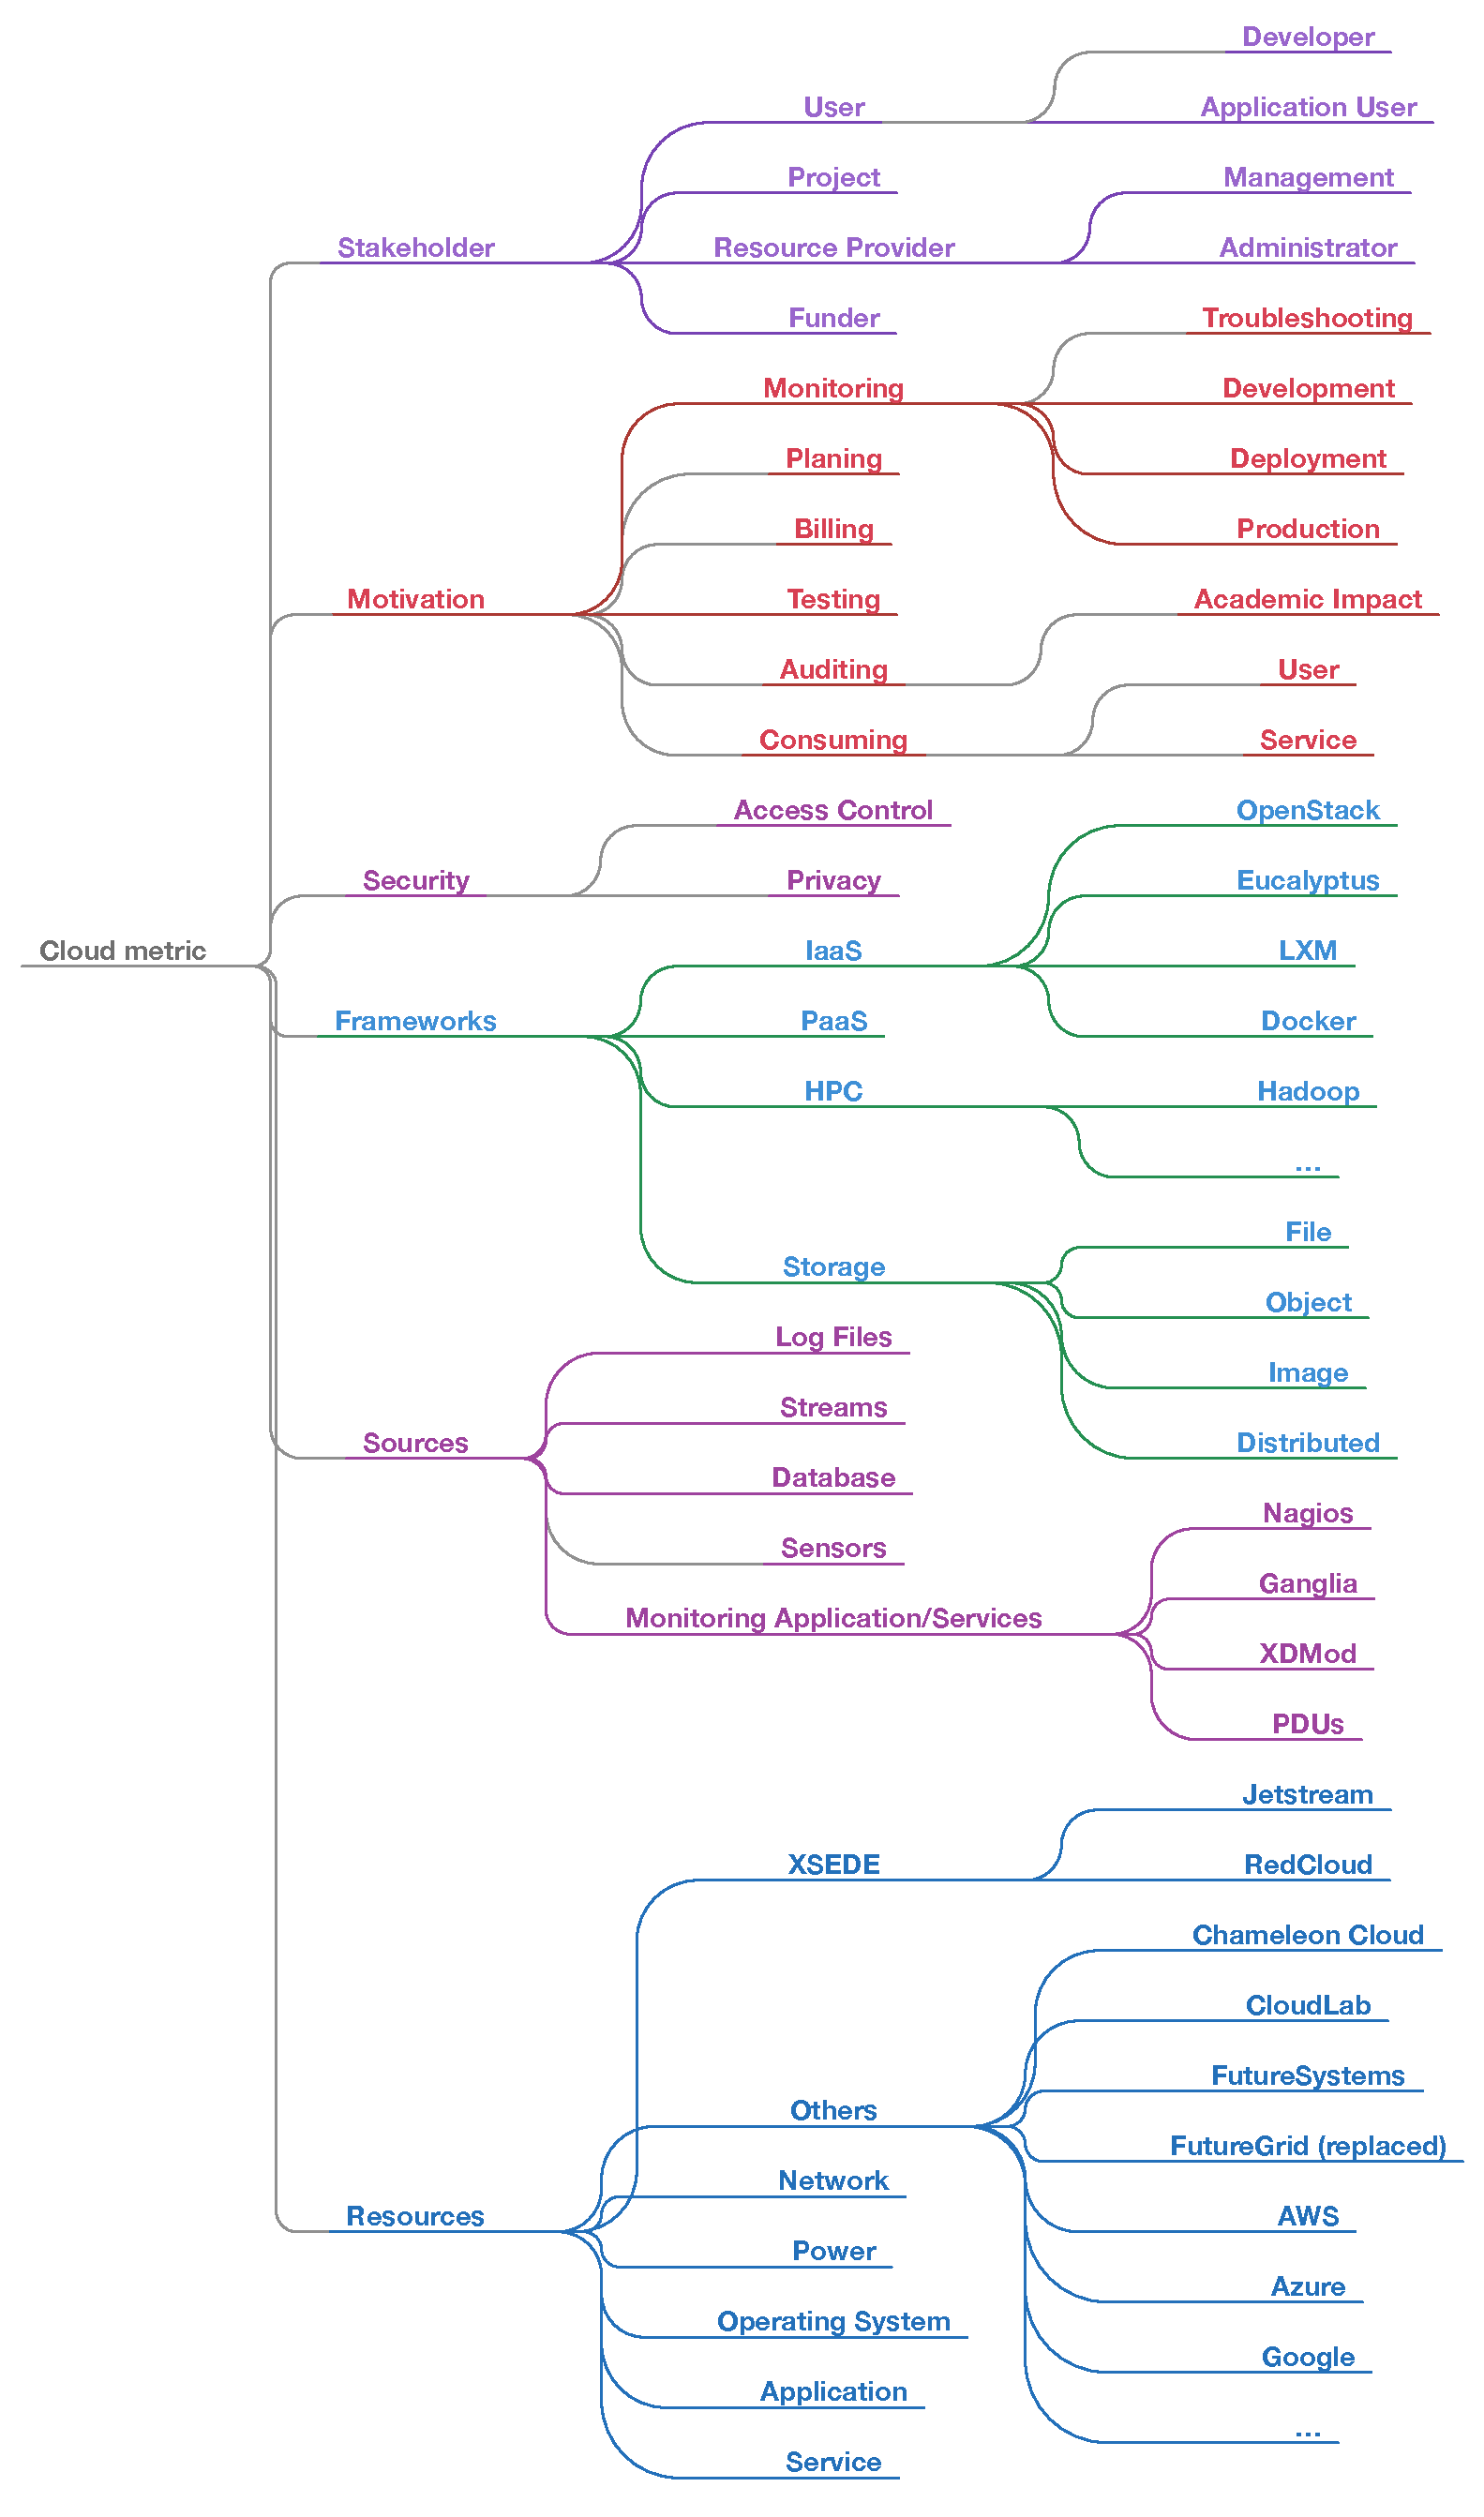
\includegraphics[width=1.0\columnwidth]{images/cloudmetric.pdf} 
  \caption{Overview of CloudMetrics}\label{F:taxonomy-1} 
\end{figure} 

\subsection{Stakeholder}

A cloud will have a wide variety of stakeholders with their
potentially specific needs in metrics. These stakeholders include (a)
the users which could be application developers and application users,
(b) a project in which multiple users contribute (c) the resource
provider including administrators and management including the
director. Furthermore, we identify the funder of the Cloud as an
important stakeholder as he may have needs for specific metrics that
are typically not relevant to users or administrators of the cloud but
have profound impact on the goal of funding the resource. To give an
example of the wide variety of metrics needed we like to make use
aware that although management is interested in operational 24/7
operation of the system and statistics associated with it, concrete
metrics and monitoring infrastructure as needed by the administrators
to detect operational failures are typically not part of the needed
metrics for a center director. On the other hand metrics to identify
ethnicity and classification into scientific disciplines are of great
value for center directors and Funders, while they play no importance
to the operational metrics to keep the system running.

\subsection{Motivation}

Another important factor for a cloud metric is the motivation and
purpose for it. We distinguish
the following factors:


\begin{description}
\setlength\itemsep{-2pt}

\item[\it Monitoring.] Monitoring is an important aspect for
  administrators but also for users. The purpose of metrics associated
  to monitoring allows us to observe the current system and make
  decisions based upon it. Naturally, this could also be services that
  act in behalf of the user or administrator. A center director may be
  interested in the high level aspects of monitoring as to be informed
  about specific catastrophic service events, while an administrator
  is interested in more detailed monitoring aspects that alert even on
  conditions that could lead to issues. Examples for monitoring
  includes measuring resource utilization in real time or over a
  period of time.  Monitoring is potentially important on all layers of
  the Cloud infrastructure from bare metal, to IaaS, PaaS, and SaaS.

\item[\it Planning.] Planing is needed to assist in setting goals and
  developing strategies several metrics can be beneficial. This
  includes metrics about utilization of the resources, satisfaction by
  the users and other more general aspects. As academic resources are
  often funded by government organizations such as NSF, specific
  metrics that answer to broader impacts need to be addressed. An
  essential ingredient of planing is the ability to include
  performance monitoring on the cloud while exposing sophisticated
  metrics.  This will enable the planing of efficient resource
  utilization from a small instance to a large virtual cluster on the
  cloud, performance management and monitoring are necessary for
  performance analysis.

\item[\it  Billing.] As academic clouds are provided free to the academic
  user community upon peer reviewed projects, it is also important to
  avoid situations that either over-stress or adversely lead to
  underutilization. For example in absence of billing against real
  monetary values, we observed that many users ignore the cost that is
  involved by running an actual VM. Furthermore, it is important to
  communicate to the users the potential estimated cost to them in
  order to educate them towards deleting or suspending unused
  resources. However, at the same time it must be assured that large
  enough experiments can be conducted to further some of the more
  challenging scientific problems.

\item[\it  Testing.] As cloud environments and they usage in applications
  may be complex (at times more complex that their HPC counter parts)
  it is important that metrics be provided that support the testing of
  the functionality, the performance, and the scalability. Ideally
  these metrics should be available as part of automatic testing
  services that however may be customized for a particular application.

\item[\it  Consuming.] Many metrics will assist the users and services to
  consume the cloud services efficiently. They will provide
  information in optimizing resource use and distribution amongst
  them. They will also alert towards limitations of the underlaying
  systems and provide insight on where application limitations my
  hinder adoption. A specific case is the creation of user motivated
  benchmarks that through their metrics can inform users about which
  cloud setup is particularly beneficial.

\item[\it Auditing.] Metrics for auditing support the process to
  evaluate the clouds design and effectiveness. This includes
  security, deployment processes, development processes and governance
  and oversight processes.  It includes finding a proof and a trait of
  actions a user made while resources are being used. Observing a
  user's, or service's behavior should be performed by logging events
  and detailed information is necessary to track back any issues on a
  system.  An important aspect or a comprehensive auditing process is
  that that it is conducted by an independent and unbiased
  observer. Auditing should not be confused with monitoring the system
  in real time.

\end{description}


\subsection{Security}

Due to targiteng different user communities it is obvious that smoe
metrics may not be exosed to all its users and are potentially unde
access control. Furthermore, users that consume cloud resources may
have the desire that their information is private and may not be
shared with other users. However, although it is possible to provide
acess and privacy controls we have seen in government agency sponsord
reserach environments a general consensus of transparency mandated by
the funding agency such as NSF. A good example here is XSEDE that
provides a great deal of information to its users. When looking at a
metic framework for clouds we need to consider the posibility to
restrict eccess through access control policies that regulate privacy
concerns. Such policies need to include role based restrictions of
stakeholders and metrics to be accessed by them.

\subsection{Frameworks}

As already pointed out in the introduction, it is important to not
isolate the cloud metrics. Although they can be developed
independently in many cases we need a larger picture for projects that
require a heterogeneous set of services and frameworks for their
scientific mission to succeed.  This includes the integration of high
performance computing resources and services (HPC), storage resources
and services, infrastructure as a service based resources build from
either OpenStack, VM Ware, or Nimbus, as well as various platform as a
service environments that enable academic users to focus on the
platform regardless of which underlaying resource framework is chosen.
Furthermore it may be important to consider extending the cloud
metrics framework to public clouds such as using AWS as this may be an
integral part of the strategy to offer services to academic users and
groups. Restrictions posed by some of these frameworks such as the
lack of groups in the Nimbus framework make it problematic to meet the
demands fro example of an academic (e.g. XSEDE) based metric
framework. Thus Nimbus must provide group support in order to become
meaningful in academic project based deployments while providing
comprehensive metrics.

\subsection{Resources}\label {S:resources}

Metrics that are implicitly provided by various cloud providers are
important for gaining a complete picture of a particular project. This
may include the following

\begin{description}
\setlength\itemsep{-2pt}

\item[\it Commercial public clouds.] These are clouds that are offered
  commercially or for free to academic users. While an individual se
  of time limited user based usage may not be of importance it becomes
  essential if actual money is paid to provide this service to
  academic users. Important may not only the amount of money paid, but
  to justify the academic and scientific impact
  \cite{las2015cluster,las2015xsede} that is derived by such efforts.

\item[\it Academic public clouds.] Recently NSF has provided a significant
  amount of funding to cloud offerings for the academic community. In
  order to justify its funding and to contrast it to commercial public
  cloud offerings metrics and evaluation criteria need to be
  developed that justify their existence. 

\item[\it Academic private clouds.] Many universities have started to
  offer private clouds to their user community, This includes not only
  the use of academic efforts, but also of production clouds to support
  the internal IT infrastructure as part of a universities management
  IT infrastructure. While in the IT department operational cost and
  privacy are potentially dominating the metrics, in academic clouds
  the se in projects and their outcome metrics need to be
  integrated. This reflects similar metrics that we find while using
  commercial and academic public clouds.

\end{description}

Examples for publicly funded clouds include XSEDE while offering HPC
services to its users, Chameleon Cloud, CloudLab, as IaaS based clouds
and network experiment infrastructure, and Jetstream as Iaas and PaaS
supporting cloud. Additionally the following Resources offered to
academic users will have a potential impact on the definition of Metrics:

\begin{description}
\setlength\itemsep{-2pt}

\item[\it MRIs.] According to the NSF web pages, the `Major Research
  Instrumentation Program (MRI) catalyzes new knowledge and
  discoveries by empowering the Nation?s scientists and engineers with
  state-of-the-art research instrumentation. The MRI Program enables
  research-intensive learning environments that promote the
  development of a diverse workforce and next generation
  instrumentation, as well as facilitates academic/private sector
  partnerships.'' Some of the MRI funding supports significant
  computational resources offered to a particular user community. In
  such cases it would be beneficial if the metrics and services
  introduced here can be reused by such efforts and adapted
  accordingly. 

http://www.nsf.gov/od/oia/programs/mri/~\cite{nsf-mri}

\item[\it Networks.] With the advent of 100GBEthernet research
  environments as provided in Chameleon cloud and XSEDE it is
  essential that network related information be integrated into an
  overarching metric framework. This includes not only details of the
  overall use of the network, but the specific information which
  projects, or even which applications are using it. Access control to
  this information may has to be investigated in order not to expose
  exploitable information to the community.

\item[\it Storage.] Obviously many cloud applications in the bid data
  area require large amount of storage either as files, databases, or
  object stores. Metrics must be available to the users and the
  providers in order to assess needs and availability. Storage has
  traditionally been an issue in academic environments.

\item[\it Power.] A significant cost in operating an academic cloud is
  power consumption. It is important that the IT departments of the
  academic cloud providers put efforts in place that power usage is
  transparently exposed so that associations between power and
  services offered can be achieved. This goes beyond the measurement
  of poer consumption within servers, but muct inclde a more
  generalized approach while integrating PDU information and other
  available metrics that may already be available. However, typically
  such information is often isolated and potentially not available to
  the academic user community without a significant effort. Future
  designs of academic datacenter should keep in mind that such
  information ought to be transparently provided to the researchers or
  retrofitted accordingly.

\item[\it Operating Systems.] Traditionally a large amount of metric
  information is available as part of the operating system either in
  virtualized or in bare metal mode. The included services can present a
  great deal of information to users and to the provider. Tools such
  as Nagios and Ganglia provide  the ability to collect and integrate
  the information sources.

\item[\it Applications.] Many academic users will develop a number of
  applications on available resources. Metrics that compare efficiency
  and effective use of such applications will be important as to
  evaluate prudent use of the resources. For example in some cases it
  may be essential to measure the performance impact of using cloud vs
  HPC resources. In other cases it may be more important to focus on
  manpower consumed to develop applications on more complex
  environments. Supporting performance APIs and libraries may aide in
  the development of metrics and their associated services such as the
  use of PAPI \cite{papi2014}.

http://icl.cs.utk.edu/papi/~\cite{papi-web}


Nelson, John "Analyzing PAPI Performance on Virtual Machines," ICL
Technical Report, ICL-UT-13-02, August, 2013.~\cite{JohnNelsonAnalyzingPAPI}

\item[\it Services.] In addition to applications we also are in the
  need of metrics provided by services offered to the community. 

\end{description}


Hyungro Report: \cite{LeeFGresource}

\subsection{Sources}

A comprehensive metrics framework consists of a data mashup of various
sources of information. It will not be sufficient to just present a
heterogeneous set of metrics to the users, but it will be desirable to
integrate several into an easy to use framework. This has been
effectively demonstrated by XDMod for HPC
\cite{las14cloudmeshmultiple,las14Impact,las12xdmod-kernel}. This was
possible due to a sustained effort within the project to provide such
integrated metrics. In the cloud IaaS area the FutureGrid project has
pioneered such an integrated framework that combined multiple sources
into an easy to use report generation framework. It was operational
for a number of years and is still actively used by the FutureSystems
project. At this time it is unknown which strategies are pursued by
projects such as chameleon cloud and other NSF sponsored projects.  In
fact there may be an advantage that such activities be continued by an
external party such as FutureSystems and be adopted by other in order
to be true to the independence of the auditing principle which need to
be employed to evaluate the effectiveness of such infrastructures


\begin{figure*}[htb] 
  \centering 
    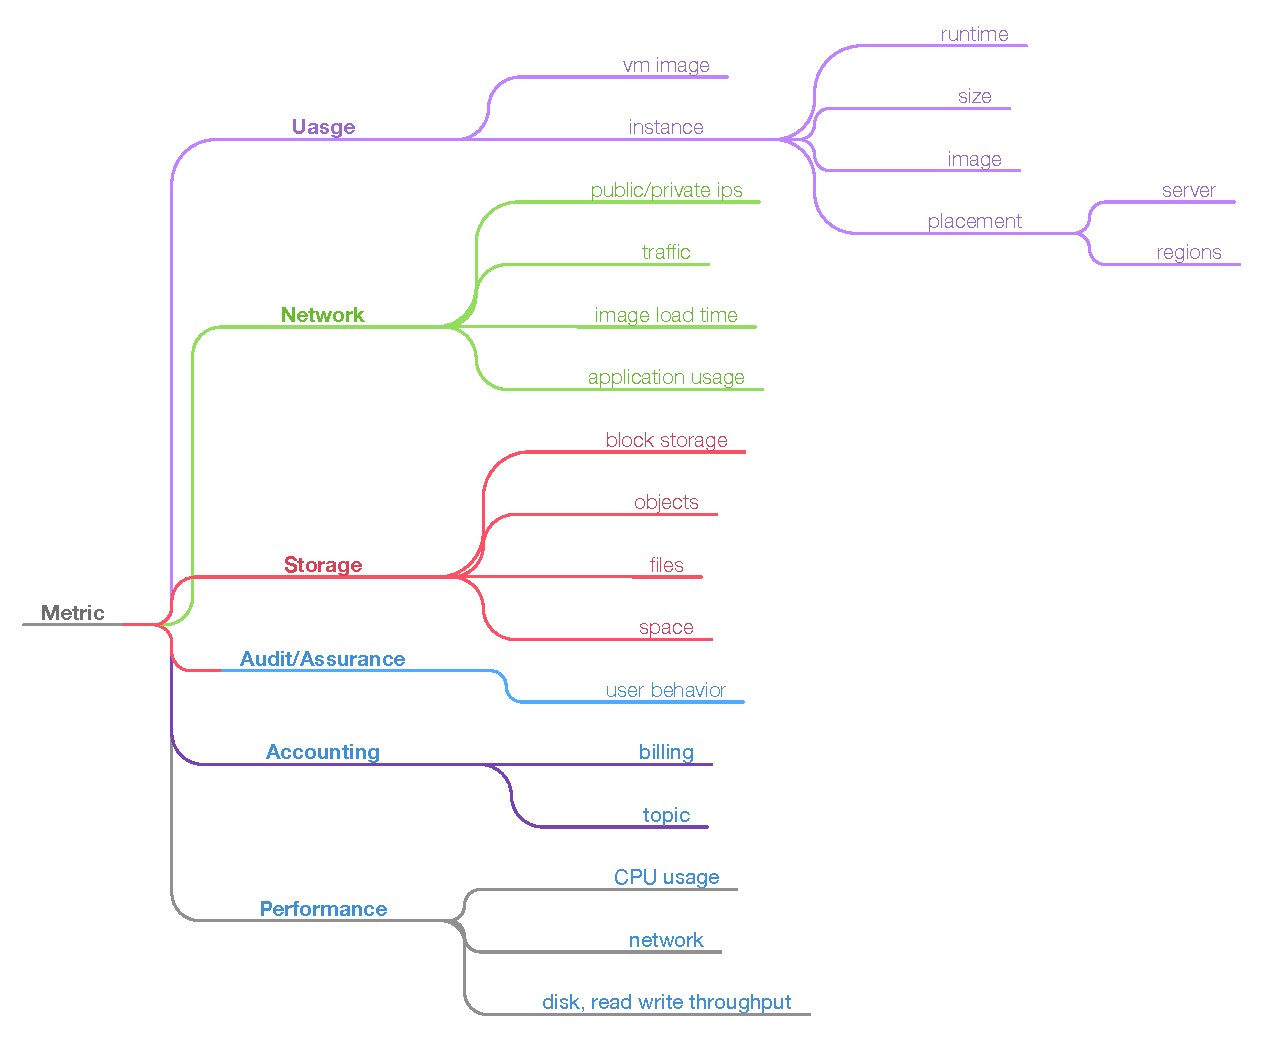
\includegraphics[width=0.6\textwidth]{images/cloudmetric-2.pdf} 
  \caption{Overview of CloudMetrics}\label{F:taxonomy-2} 
\end{figure*} 



%%%%%%%%%%%%%%%%%%%%%%%%%%%%%%%%%%%%%%%%%%%%%%%%%%%%%%%%%%%%%%%%%%%%%%
\section{CLOUD METRICS} \label{S:metrics}
%%%%%%%%%%%%%%%%%%%%%%%%%%%%%%%%%%%%%%%%%%%%%%%%%%%%%%%%%%%%%%%%%%%%%%


\subsection{Summary Report (All)}

                                                                                       
format, table, piechart, barchart, stacked barchart, period month quarter, week day, hour current                                       

\begin{verbatim}
o       1.1  WallHoursbyClusters(Total,monthly)
o       .2  VMCountbyClusters(Total,monthly)
o       1.3  UsersCountbyClusters(Total,monthly)
o       
o       VMs count, Users count, Wall hours, Distribution by Wall Hours, Project, Project Leader, and Institu- tion, and Systems 

\end{verbatim}

\subsection{Summary (Monthly) }

\begin{verbatim}
o       put multiple metrics in same chart
o       period y, m, d, h                                                                                                
o       Metrics: VMs count, Users count, Wall time (hours), Distribution by wall time, project, project leader, and institution, and systems 
        system information on which hosts do we run, count vms, runtime
\end{verbatim}

\subsection{Keywords}

\begin{Verbatim}[fontfamily=times]
o usage
   -   VM image
   -   instance
o runtime
o size (flavor)
o image
o regions
   -   network
o public/private ip address
o traffics
   -   storage
o block storage
o objects
o files
o space
o audit/assurance
  -   user behavior
o server utilization
o errors
  - detect incidents
  - trace issues/ bugs
  - prevent long downtime
o billing/charging/accounting
o commercial monitoring services
  - openstack ceilometer / telemetry
  - aws cloud watch
  - google cloud monitoring beta
o performance
  - cpu usage (utilization) 
  - network in/out bytes
  - disk read/write throughput
  - power consumption
  - memory usage
  - latency (e.g. network response or vm start)
o monitoring service
  - alert/notification (e.g. text, email)
  - diagnostics
  - security
  - capacity planning/prediction
  - trend changes
o Physical hardware monitoring
  - host contention
  - degraded hardware
  - outages
  - downtime
o automation
  - recovery
  - autoscaling
  - policy/threshold to take actions
  - live migration
o monitoring frequency
  - real-time
  - interval
  - lifespan of measured data
o Consideration of Cloud Metrics
  - architecture
  - overhead
  - security/privacy
  - interface
o rest api
o dashboard
o management console
  - visualization
o charts
o time series data
o consideration of implementing metrics system
  - scalability
  - overhead
  - availability
  - accuracy
  - security
  - agility
  - autoscaling
\end{Verbatim}

\begin{verbatim}
o  VM
o  Usage
o  Failure
o  Prediction
\end{verbatim}

\begin{verbatim}
Total User Count
Count over Group
Project, Center, Organization
Counts the active users in the cloud
\end{verbatim}


\begin{table*}[htb]

\caption{Metrics Table}
\begin{scriptsize}
\label{T:metrics}
\bigskip
\begin{tabular}{lp{0.1\textwidth}p{0.1\textwidth}p{0.3\textwidth}p{0.3\textwidth}p{0.1\textwidth}}
ID & Name & Stackeholder & Description & Motivation & Sample \\
\hline
UC.1&
User Count & 
~&
This metric counts the active users for the cloud &
User count is important for measuring the popularity of the cloud & 
Reports (Fig~1,~2) \\
\hline
VC.1&
VM Count & 
~&
This metric counts the launched VM instances on the cloud &
VM Count is important for measuring the volume of requested instances &
Reports (Fig~1,~2) \\
\hline
RS&
Runtime Sum&
~&
This metric shows the total amount of runtime for launched instances &
runtime by hour is important for measuring actual runtime of instances &
Reports (Fig~1,~2) \\
\hline
VC.2&
VM Count by Project, Leader, or Institution &
~&
This metric shows share of resource by group metrics such as project, leader or institution &
Group usage is important for measuring group usage &
Reports (Fig~1,~2) \\
\hline
VC.3 &
Current running VMs or accessed users &
~&
This metric shows instant usage data to see current status &
real time usage is important for checking peak or detecting unusual usage &
Reports (Fig~1,~2) \\
\hline
\end{tabular}
\end{scriptsize}
\end{table*}

ID
realtime
stakeholder = user, administrator, management, funder
type = count, sum, distribution, ....

Fig 1. Active user count by host                  

Fig 2. Active user count monthly

Fig 3. VM Count daily
 
Fig 4. VM Count by runtime distribution

Fig 5. Usage by Institution
 
Fig 6. runtime by Hour by Project Leader

Fig 7. Real-Time Usage of VM instances
 
Fig 8. Real-time userlist of running VM instances

\subsection{Sample Reports}

FutureGrid html \cite{LeeFGresourceWeb}
 FutureGrid pdf \cite{LeeFGresource}

\subsection{Report for Errors (TBD)}

Cloudmesh Metrics reads system and application logs to generate error reports. If there are error messages stored in the database, Cloudmesh Metrics can lookup the database to collect the messages. Error information collected are stored in the Metrics database.

\subsection{Possible Analysis (TBD)}

There are possible metrics to measure based on the observation of error messages on cloud platforms, especially OpenStack.

\begin{verbatim}
o  Identify problematic hosts
- e.g. 20% of errors occurred in i57
o  Identify problematic term
o       e.g. 46% of errors occurred in April 2014
o  Identify errors with a hierarchical classifier
o       1st level: code
o       2nd level: message
o       3rd level: Python exceptions
o       e.g. 88% of errors occurred in 500 code and 33% of the errors were due to invalid instance types: “Instance type's disk is too small for requested image.”
o       1st level
Code Number     \# of Errors
400     12
404     4
409     41
500     399

o       2nd level
\end{verbatim}

\hyungro{transfer tables here and eliminate the verbatim} 

\begin{verbatim}
Code Number     Message \# of Errors
500     'NoneType' object has no attribute 'defineXML'  

        1
        Instance type's disk is too small for requested image.          133
        No valid host was found.        93
        Unable to read from monitor: Connection reset by peer   126
        Unexpected error while running command. 11
        Requested operation is not valid: domain is already running     1
        ...     

o       3rd level (for debugging error messages)


Code    Message Parsing Details - Python Module Parsing Details - Python Function       \# of Errors
500     Instance type's disk is too small for requested image.  nova/compute/manager.py \_build\_instance()     133
...                             

\end{verbatim}

\begin{verbatim}
o  Error rate
-       e.g. 1.5 % error rate on nova-api requests on 03/25/2014
(based on nova-api.log-20140325: 17338 accepted requests and 266 errors)
o  Audit information (nova-compute)
-       Resource tracking
-       e.g. available/free disks, memories or vcpus
o  Error Tracing
-       e.g. nova.api.ec2 (/services/Cloud/) has “Unexpected TypeError raised” with a user from 128.9.136.58

o  Possible other metrics (TBD)
o  quota management
o  alert notification
\end{verbatim}


\subsection{Extra tables}

\hyungro{introduce begin center and center in all tables}
\hyungro{lets use scriptsize in all tables, this way they look uniform}

\begin{table*}[htb]

\caption{Basic Concept of Metric}
\label{T:BCmetrics}
\bigskip
\begin{tabular}{p{0.1\textwidth}p{0.1\textwidth}p{0.3\textwidth}p{0.4\textwidth}}
Name & Unit & Type of Value & Refresh Interval (Measuring time) \\
\hline
Runtime &
hour, min, sec &
cumulative,
aggregation &
event-triggered \\
\hline 
running jobs &
count &
delta, 
(change from the previous value) &
time-triggered e.g. 5 secs, 5 mins\\
\hline
CPU, Memory, Load &
Percentage &
gauge,  
(standalone value relating only to the current duration) &
time-triggered e.g. 5 secs, 5 mins\\
\hline
\end{tabular}

\end{table*}


\begin{table*}[htb]

\caption{System Performance Metric (OS Level)}
\label{T:SPmetrics}
\bigskip
\begin{tabular}{p{0.1\textwidth}p{0.1\textwidth}p{0.1\textwidth}p{0.1\textwidth}p{0.1\textwidth}p{0.1\textwidth}}
Metric & Description & Type & Level & Unit & Example \\
\hline
CPU Utilization &
Percentages of total CPU time &
System Monitoring &
Operating System & 
Percentage & 
vmstat \\
\hline
I/O Read &
Read operations on disks &
&
&
Count or Bytes &
iostat \\
\hline
I/O Write &
Write operations on disks &
&
&
Count or Bytes  &
\\
\hline
Network In &
Received bytes to network interfaces &
&
&
Bytes &
\\
\hline
Network Out &
Sent bytes from network interfaces &
&
&
Bytes &
\\
\hline
\end{tabular}
\end{table*}


\begin{table*}[htb]
\caption{Network Monitoring Features (source from wikipedia)}
\label{T:NMmetrics}
\bigskip
\begin{tabular}{p{0.1\textwidth}p{0.3\textwidth}p{0.1\textwidth}p{0.1\textwidth}}
Metric (legend) & Description & Ganglia & Nagios \\
\hline
Trending &
provides trending of network data over time &
Yes &
Yes \\
\hline
Trend Prediction &
The software features algorithms designed to predict future network statistics &
No &
No \\
\hline
Auto Discovery &
The software automatically discovers hosts or network devices it is connected to &
Via gmond check in &
Via Plugin \\
\hline
Agentless & 
The product does not rely on a software agent that must run on hosts it is monitoring so that data can be pushed back to a central server. &
No &
Supported \\
\hline
SNMP &
able to retrieve and report on SNMP statistics &
via plugin &
Via plugin \\
\hline
Syslog &
Able to receive and report on Syslogs &
No &
Via plugin \\
\hline
\end{tabular}
\end{table*}


\begin{table*}[htb]
\caption{Metrics for Cloud Computing}
\label{T:NMmetrics}
\bigskip
\begin{tabular}{p{0.1\textwidth}p{0.2\textwidth}p{0.1\textwidth}p{0.1\textwidth}}
Metric & Cloud Platform & Purpose & Related Service \\
\hline
CPU Utilization &
IaaS, PaaS &
Performance &
Scale Up/Down \\
\hline
Task completion time &
PaaS &
Performance &
\\
\hline
Number of VMs &
IaaS &
Traffic &
Scale Up/Down \\
\hline
VM sizes (flavors) &
IaaS &
Capacity &
\\
\hline
\end{tabular}
\end{table*}
\cite{aceto2013cloud}

\begin{table*}[htb]
\caption{System Monitoring on Cloud platforms}
\label{T:SMmetrics}
\bigskip
\begin{tabular}{p{0.1\textwidth}p{0.1\textwidth}p{0.1\textwidth}p{0.1\textwidth}p{0.1\textwidth}p{0.1\textwidth}p{0.1\textwidth}}
Metric & AWS & GCE & Azure & OpenStack & HP Cloud (Eucalyptus) & Nimbus \\
\hline
CPU Utilization & Yes & TBD & TBD & TBD & TBD & TBD \\
\hline
I/O Read & Yes & TBD & TBD & TBD & TBD & TBD \\
\hline
I/O Write & Yes & TBD & TBD & TBD & TBD & TBD \\
\hline
Network In & Yes & TBD & TBD & TBD & TBD & TBD \\
\hline
\end{tabular}
\end{table*}

%%%%%%%%%%%%%%%%%%%%%%%%%%%%%%%%%%%%%%%%%%%%%%%%%%%%%%%%%%%%%%%%%%%%%%
\section{MONITORING TOOLS AND SERVICES}\label{S:tools}
%%%%%%%%%%%%%%%%%%%%%%%%%%%%%%%%%%%%%%%%%%%%%%%%%%%%%%%%%%%%%%%%%%%%%%

\subsection{IaaS}

\subsubsection{OpenStack}

In late 2012, OpenStack community started a new project about measuring usage data from openstack components. This project named Ceilometer collects measurements within OpenStack to achieve monitoring and metering purposes. Ceilometer acquires all of the measurements across all current OpenStack components such as Nova (compute), Network, and Storage (swift), etc and provides a unique framework for the collected data. The latest release Havana includes Ceilometer as a mandatory component in OpenStack and the previous release Grizzly included it as an incubator component.

OpenStack Compute (nova) also provides a command line tools to retrieve usage statistics, for example, 'nova usage-list' provides usage data for all tenants. These management commands typically limited to system administrators to execute.

\paragraph{Ceilometer}

Ceilometer project is a framework for monitoring and metering the OpenStack cloud and Ceilometer is a primary place to get access of all usage data in openstack components. It was mainly developed to charge customers as a billing system. Like other commercial cloud platforms, for example Amazon Web Services, these metrics are included, with an hour level granularity:
  compute utilization;
   instance type;
   availability zone;
   cpu core;
   memory size;
   nova volume block device type and availability zone;
   Network;
   data transfer (in / out), availability zone;
   external floating ip;
   Storage (Swift);
   disk size used;
   data in/out.

\subsubsection{Implementation}

\task{Wrong section heading}

There is a program named an agent on each OpenStack node and aggregates information about virtualized resources. The agent on each nova compute node uses Linux virtualization API (libvirt) and Windows Management Instrumentation (wmi) to extract essential information from hypervisor. Some other agents harvest the data from iptables, swift proxy or the nova database, if additional information can be obtained through these external services.

There are four basic components to Ceilometer:

\begin{itemize}
  \item Agent: runs on each compute node and polls for resources utilization statistics.
  \item Collector: runs on management servers to manage the message queues for data coming from the agent. Metering data are stored to the openstack data store directly and a notification message are delivered to the Openstack messaging bus once it is processed.
  \item Data store: is a place of collected data. It provides interaction with the collector and a api server.
  \item API server: runs on management servers to provide statistics about the measured data.
\end{itemize}

An API server provides access to metering data in the database via a REST API. A central agent polls utilization statistics for other resources not tied to instances or compute nodes. There may be only one instance of the central agent running for the infrastructure. A compute agent polls metering data and instances statistics from the compute node (primarily the hypervisor). Compute agents must run on each compute node that needs to be monitored. A collector monitors the message queues (for notifications sent by the infrastructure and for metering data coming from the agents). Notification messages are processed, turned into metering messages, signed, and sent back out onto the message bus using the appropriate topic. The collector may run on one or more management servers. A data store is a database capable of handling concurrent writes (from one or more collector instances) and reads (from the API server). The collector, central agent, and API may run on any node. These services communicate using the standard OpenStack messaging bus. Only the collector and API server have access to the data store. The supported databases are MongoDB, MySQL, PostgreSQL, HBase and DB2; however, A dedicated host for storing the Ceilometer database is recommended, as it can generate lots of writes. Production scale metering is estimated to have 386 writes per second and 33,360,480 events a day, which would require 239 Gb of volume for storing statistics per month~\cite{Barcet12}.

Openstack itself has notification systems built into the existing OpenStack components. Most usage data are collected from these notification systems. Ceilometer also requests metering messages from a pollster plugin using the 'ceilometer.poll.compute' namespace.

\paragraph{Ceilometer with OpenStack Heat for autoscaling}

The OpenStack Orchestration program, Heat, provides an autoscaling service with Ceilometer like Amazon CloudFormation. OpenStack Heat scales VM capacity up or down according to the metrics from Ceilometer. Ceilometer collects metrics for virtual machines and its alarming module calls the Heat API if the threshold for the metrics is reached. Heat triggers the upscaling or the downscaling virtual machines once it is notified by Ceilometer. This integration of Heat and Ceilometer allows you to ensure optimal utilization by managing the number of virtual machine instances. Amazon has a similar combination of AWS Auto Scaling and AWS CloudWatch to provide the autoscaling service based on monitoring values~\cite{Abaakouk13}.

\paragraph{Nova command line tools for usage statistics}

Openstack provides usage statistics for OpenStack Compute (Nova), a main component for provisioning and managing virtual machines, with command-line tools. Simple commands displays basic statistics on resource usage for hosts (physica nodes) and instances (virtual objects running on the host). Basic information such as CPU, memory, and disk usage are viewed. These information about allocated resources to the instances do not indicate resource usage on the physical host. For more detailed information about resource usage, Ceilometer has rich functions to see user related or system related usage data. Ceilometer is available on OpenStack Hanava and Grizzly version. 

\begin{figure}[htb]
\begin{scriptsize}
\begin{verbatim}
    $ nova host-describe sierra
    +--------+------------+-----+-----------+---------+
    |  HOST  | PROJECT    | cpu | memory_mb | disk_gb |
    +--------+------------+-----+-----------+---------+
    | sierra | (total)    | 8   | 32176     | 144     |
    | sierra | (used_max) | 6   | 12288     | 120     |
    | sierra | (used_now) | 6   | 12800     | 120     |
    | sierra | project1   | 3   | 6144      | 60      |
    | sierra | project2   | 2   | 4096      | 40      |
    | sierra | project3   | 1   | 2048      | 20      |
    +--------+------------+-----+-----------+---------+
\end{verbatim}
\vspace{-20pt}
\end{scriptsize}

\caption{Display a summary of resource usage of the devstack-grizzly host}
\label{F:host-describe}

\end{figure}

Usage data can be provided by Tenant Id which is a group of openstack cloud users. Each tenant id represents a group or an account to the group members, so usage data for the tenant id are aggregated. 

\begin{figure}[htb]
\begin{scriptsize}
\begin{verbatim}
    $ nova usage-list
    Usage from 2014-02-14 to 2014-03-15:
    +--------+---------+-------------+---------+-----------+
    | Tenant | Instan- | RAM         | CPU     | Disk      |
    | ID     | ces     | MB-Hours    | Hours   | GB-Hours  |
    +--------+---------+-------------+---------+-----------+
    | user1  | 17      |  6840394.43 | 3340.04 |  66800.73 |
    | user2  | 17      |   185683.06 |   90.67 |   1813.31 |
    | user3  | 1       |   932256.36 |  455.20 |   9104.07 |
    | user4  | 26      |  4947215.08 | 2415.63 |  48312.65 |
    | user5  | 5       | 18644854.23 | 9103.93 | 182078.65 |
    +--------+---------+-------------+---------+-----------+
\end{verbatim}
\vspace{-20pt}
\end{scriptsize}

\caption{Summary statistics for tenants}
\label{F:host-describe}

\end{figure}


Usage data for Ceilometer and the nova command line tools is provided by OpenStack Notification System. The notification system can be configured to emit events either through nova's logging facility, or send them to a series of AMQP queues (one per notification priority). System usages are emitted as notification events with the INFO priority. Different types of usage events are distinguished via the notifications' 'event\_type, which is a hierarchical dotted string such as compute.instance.create, which allows usages to be easily grouped for aggregation. Usage notifications can be immediate, created when a specific increment of usage occurs (such as creation of an instance) or periodic, generated by a periodic task, like a cron job, and covering usage for a certain period of time. Besides the standard Nova Notification priority, notification timestamp, and event\_type, usage notifications contain a payload of data that will vary depending on the event\_type. This is presented as a json-formatted hash of key-value pairs. Some of the keys, such as tenant\_id will always be present in any usage notification, others will be data relevent to that event\_type (for example, instance related notifications will contain data describing the instance)~\cite{SystemUsageData}.

\subsubsection{Eucalyptus}

The Eucalyptus Amazon compatible private cloud has provided resource usage information through external monitoring tools such as Nagios and Ganglia. Since both Nagios and Ganglia have been proved to observe state data within distributed systems, Eucalyptus relied on integration with these tools for resource monitoring. To enhance system management, Eucalyptus recently improves summary reports about resource allocation and status. There are commands line tools for generating reports for eucalyptus cloud that start with eureport- in the Cloud Controller (CLC) and eucadw- in the data warehouse. The reports provide usage data for understanding how cloud resources are utilized and being used via simple command line tools. eureport-generate-report is a main command to get access usage data. Various type of resources can be measured such as elastic-ip, instance, s3, snapshot, and volume when eureport-generate-report is ran with a report type option. The Eucalyptus data warehouse is a place to keep all usage data coming from CLC. External programs can get access to the usage data from the data warehouse instead of CLC directly. It may reduce impact of pulling usage information from cloud when it performs its cloud duties~\cite{Euca2ools14}.

Regarding to commercial clouds, usage data is provided to cloud services running under your account.

\subsubsection{Azure}

Microsoft Azure - Microsoft Windows Azure is a cloud computing platform used to build, host and scale web applications through Microsoft data centers~\cite{azure11}. The platform contains various on-demand services hosted in Microsoft data centers. These services are provided through three products.

\begin{itemize}
 \item Windows Azure: an operating system that provides scalable compute and storage facilities.
 \item SQL Azure: a cloud based, scale out version of SQL server.
 \item Windows Azure AppFabric: a collection of services supporting applications both in the cloud and on premise.
\end{itemize}

The System Center Monitoring Pack for Windows Azure application is the most cost effective and flexible platform for managing traditional data centers, private and public clouds, and client computers and devices~\cite{MonitoringPackAzure11}. It provides monitoring of availability and performance for Windows Azure applications. It is the only unified management platform where multiple hypervisors, physical resources, and applications can be managed in a single offering. From a single console view, the IT assets like network, storage and compute can be organized into a hybrid cloud model spanning the private cloud and public cloud services.

The monitoring pack runs on a specified agent and uses Windows API.s to remotely discover and collect information about a specified Windows Azure application. By default, the monitoring is not enabled. Therefore, the discovery must be configured by using the Windows Azure Application monitoring template for each Windows Azure Application to be monitored.

The following functionalities are provided by the Monitoring Pack for Windows Azure Applications:

\begin{itemize}
 \item Discovers Windows Azure applications.
 \item Provides status of each role instance.
 \item Collects and monitors performance information.
 \item Collects and monitors Windows events.
 \item Collects and monitors the .NET Framework trace messages from each role instance.
 \item Grooms performance, event, and the .NET Framework trace data from Windows Azure storage account.
 \item Changes the number of role instances.
\end{itemize}

Implementing monitoring means, launching the diagnostic instance and this instance will collect the data and at the interval user wants. The collected data will be copied to an Azure Table:

\begin{itemize}
\item WADPerformanceCountersTable for the performance counters
\item WADWindowsEventLogsTable for the windows event logs.
\end{itemize}

The performance monitoring can be enabled by implementing some code or using some tools like:

\begin{itemize}
  \item Powershell cmdlets for Windows Azure~\cite{cmdlets}
  \item Azure Diagnostics Manager 2 from Cerebrata~\cite{cerebrata}
\end{itemize}

By using these tools one instance of Windows Azure is configured to collect some performance counters without modifying the application code. The performance data will be collected by the Azure Diagnostic Monitor and moved at the interval user specified to a table called WADPerformanceCounters. User can use diagnostic data for debugging and troubleshooting, measuring performance, monitoring resource usage, traffic analysis and capacity planning, and auditing. Diagnostic data is not permanently stored unless user transfers the data to the Windows Azure storage emulator or to Windows Azure storage. After the data is transferred to storage it can be viewed with one of several available tools. To collect Windows Event logs in a Windows Azure application, the Event logs data source must be configured.

Once, the Azure Management Pack is installed, three .run as. accounts must be created in System Center Operation Manager:

\begin{itemize}
 \item One for binary authentication. This account will use the management certificate to connect to Azure.
 \item One for basic authentication. This account will be used for the certificate
 \item One that will be used for the proxy agent.
\end{itemize}
 
The monitoring data can be visualized using System Center Operation Manager Console. From Operation Manager, user can create custom dashboard or publish graphs on SharePoint to people who do not have the SCOM console.

\subsubsection{Amazon}

\paragraph{Amazon CloudWatch}

Amazon CloudWatch monitors your Amazon Web Services (AWS) resources and the applications you run on AWS in real-time. ACW is a metrics repository. AWS product puts metrics into the repository, and users retrieve statistics based on those metrics. Metric is a variable you want to measure for your resources and applications. Namespaces are containers for metrics. Metrics are time-ordered sets of data points, are isolated from one another in different namespaces so that metrics from different applications are not mistakenly aggregated into the same statistics. Users retrieve statistics about those data points as an ordered set of time-series data. Over the time value is important for metrics since it contains historical changes in it. Timestamp always follows with a metric. Amazon provides PutMetricData API to create a custom metrics and publish to ACW. 2 weeks time period for store statistics. Each metrics has a dimension, which is a name / value pair that helps you to uniquely identify a metric.

CloudWatch has a notification to alert users and auto scaling (automatically make changes) to the resources you are monitoring based on rules that you define. Simply, CloudWatch manages threshold values to send a notification to users via email or text messages, and even more, apply changes with a pre-defined settings such as increasing virtual instances or diminishing. You gain system-wide visibility into resource utilization, application performance, and operational health.

\subsubsection{Rackspace Cloud Monitoring}

Rackspace Cloud Monitoring is an API driven monitoring system which allows administrators to use or create APIs depending on their needs which can send notifications to any device including mobile devices. This allows administrators to be on top of their Rackspace-hosted infrastructure which includes websites, protocols, and ports.

\subsubsection{Google Cloud}

Stackdriver provides monitoring service at Google Cloud

\task{Add a section to describe monitoring on Google Cloud}

\subsection{HPC}

Monitoring in high-performance computing has a similarity to Cloud Computing. It provides fixed number of jobs that a user can create and each job runs on a same size of nodes in clusters. There are also common management tools to clusters, so accounting data can be collected from these tools.

\subsubsection{XDMoD}

XDMoD (XSEDE Metrics on Demand)
\cite{las14cloudmeshmultiple,las14Impact,las12xdmod-kernel} is
primarily developed as UBMoD (University Buffalo Metrics on Demand)
and is an open source tools for collecting and mining statistical data
from cluster resource managers such as Torque/Maui, OpenPBS, SGE and
Slurm commonly found in high-performance computing environments. There
are three fundamental components: a metrics repository (XDMoD Data
Warehouse), a RESTful API, and a web-based application (XDMoD
Portal). Its web graphical user interface, XDMoD Portal, provides rich
set of statistics with different type of charts and tables with
communicating its RESTful
API.~\cite{CPE:CPE2871,Furlani:2013:UXF:2484762.2484763}\hyungro{identify
  duplicated refeneces and remove them, remember to use vonLazewski
  refs from the vonLaszewski-jabref.bib file}
 

\subsubsection{Nagios}

Nagios is a web based Linux monitoring systems and it allows to monitor availability and response time of network services, usage of system resources like CPU load, RAM allocation etc., number of logged in users and so on. The main Nagios instance (server) collects information from Linux, BSD, Windows hosts or Cisco devices through Nagios clients (agents), and sees states of their services or processes in one place: Nagios web interface. Nagios generates a notification in case of any outage detected or any anomaly through wide range of alert methods such as e-mail, sms, chat messages and phone call notifications. And one more thing, Nagios monitors states but it doesn.t show any graphs like network interface usage etc.

\subsubsection{Cacti}
Cacti is a network monitoring tool using simple network management protocol (SNMP) and similar to other tools such as Nagios and Ganglia, it uses RRDtool as a DBMS and a visualization graphical tool. Since it supports polling monitoring data via shell scripts like php or c-based executable, it can be extended to measure other resources not only network traffic. It is also suitable for a hosting service with user-based management.

\subsubsection{Zabbix}

Zabbix is an open source monitoring not only for networks but also for servers using SNMP, IPMI, and JMX. The centralized server of Zabbix collects monitoring data through several Zabbix agents installed on desirable hosts and store them on the database to display and generate web-based reports when they are needed. Zabbix Agent which is deployed on a monitoring target obtains utilization data using various monitoring protocols and tools like SNMP, TCP, and ICMP. For the cloud monitoring, Zabbix active agent auto-registration helps monitoring cloud instances such as Amazon cloud, and OpenStack without configuring manually.

\subsubsection{Zenoss}

Zenoss (Zenoss Core) provides a unified resource management service which manages applications, networks, servers, and storage in terms of monitoring physical or virtual systems including the public, private and hybrid cloud. It is built on the Zope object-oriented web application server, and using RRDtool with MySQL as to store collected information using SNMP, SSH, WMI and log files e.g. syslog. Zenoss provides additional features with other monitoring mechanisms such as Perfmon, JMX, and VM API (e.g. VMware API) in the enterprise version which is based on the open-source core version. The one of the key features of Zenoss is Model-Driven Monitoring which is about automatic and dynamic discovery, configuration and monitoring. As a communication tool, Zenoss utilizes Twisted Perspective Broker (PB) instead of AMQP typed messaging system like RabbitMQ. They claims Twisted provides an asynchronous, event-driven with co-operative multi-tasking which is a deferred object.


\subsubsection{Inca}

Keenland, Darter, FutureGrid

\hyungro{add information}

\subsubsection{Ipm} Stempede

\hyungro{add refs}
http://projekt17.pub.lab.nm.ifi.lmu.de/ipm/publications.html

https://github.com/nerscadmin/ipm

\cite{ipm10}

\subsubsection{PAPI}

\hyungro{add refs}
\task{add information} Stempede

\subsubsection{Gold}

There is a small number of accounting software to provide metered
resource utilization in open source cloud platforms. Those tools such
as Gold accounting Manager~\cite{jacksongold} are very simple and are
supposed to support system administrators not cloud users. 

\improve{Gold is no longer supported}

\hyungro{add refs}
http://docs.adaptivecomputing.com/gold/

\subsubsection{XRAS}

\hyungro{add refs}
\begin{verbatim}
http://www.researchgate.net/publication/264737715_XRAS_Allocations_software_as_a_service_in_XSEDE
\end{verbatim}

%%%%%%%%%%%%%%%%%%%%%%%%%%%%%%%%%%%%%%%%%%%%%%%%%%%%%%%%%%%%%%%%%%%%%%
\section{CLOUDMESH METRICS SERVICES AND FRAMEWORK}\label{S:cloudmesh}
%%%%%%%%%%%%%%%%%%%%%%%%%%%%%%%%%%%%%%%%%%%%%%%%%%%%%%%%%%%%%%%%%%%%%%

Cloudmesh Metrics is a plugin of Cloudmesh, Cloud management software for handling multiple cloud platforms, to provide measurement of usage data about cloud resources. It collects usage data directly from multiple cloud management nodes and provides a single usage report. 3 cloud platforms and 5 regional hosts were included in the FutureGrid project, for instance, Eucalyptus, OpenStack, and Nimbus were supported and India, Foxtrot, Hotel, Sierra, and Alamo were included. Use of Cloud Computing is leasing resources. A user requests computing resources and a cloud provider allocates requested resources from virtualized environments. At the same time, the cloud resources allocated to users e.g. virtual machine instances are recorded in database or application logs in most cloud platforms and Cloudmesh Metrics generates cloud usage reports based on the recorded data on a cloud provider. The native usage data from different clouds are integrated into the Metrics database (MongoDB is used) and the analyzed usage data are accessible in different formats such as Rest API, CLI, PDF or HTML. The web interface displays the usage data in highcharts, the javascript charting framework, with various chart types such as bar, line or pie to represent numerical data with symbols. The PDF report contains several graphical charts with tables for the detail numbers in several timelines e.g. weekly, monthly, quarterly or yearly. 
  
\improve{ Eucalyptus 2.0 and 3.0 Enterprise generates resource usage
  information via log messages with user information. We have an idea
  for a log parsing tool to collect metering values from Eucalyptus
  and a command line tool to show measured data. A graphical
  representation of measured data is required to represent multiple
  numbers of numerical metrics and we have chosen
  HighCharts~\cite{highsoft2012highcharts}, Google Chart API to
  generate chart images.  }

\subsection{Overview}
In distributed systems and HPC, resource usage are typically monitored to detect any hardware and software issues. Real-time monitoring applications help provide sustain and consistent services and engage performance of their system. Distributed systems were built with complex hardwares and require to incorporate with various hardwares such as router, switch, network, and servers along with computing resources like cpu, memory and disk. In Cloud Computing, people have attention to monitoring and accounting systems in virtualized environments, so that they can measure resource consumption which is what they are paying for on the on-demand service, cloud computing. 

Many places now adopt virtualization and cloud services to enhance the capacity of their system infrastructure and performance. Performance management is getting more important in this regard for identifying and delivering reasonable resource allocation. But traditional performance software are still designed to measure a certain type of resources and system administrators raised needs for a unified performance management with virtual resource allocation which provides a bird eye's view to monitor system utilization with the proper provision and allocation of resources~\cite{Habibzai12}. The unified monitoring software is not only about an integrating metric units and aggregating numerical values but also about making sure that the applications on the services are efficiently consuming allocated resources and the resources are properly allocated in the right place at the right time. Understanding system utilization and application performance with the observation from the software is important to satisfy service-level agreements (SLAs) and improve the system administration, however in a virtualized environment, measuring shared resources is not an easy task since they are in multiple points and different layers. 


\subsection{Real Consumption vs Allocation}
There are two types of measuring resource usage on the cloud. Like a conventional monitoring, resource consumption on the cloud is based on current usage data for cpu, memory, network and disk traffics. These are dynamically changing according to traffics, and are important to validate system health frequently. The other type of measuring resource usage is measuring the amount of allocated resources. It is an accounting system that records allocation of resources. In a shared resource environment which is a fundamental concept in utility computing, the amount of allocated resource means that your requested resource will be dominated to you not interrupted by any other users. Resource allocation is not measuring real-time resource usage. Instead, it records rented resources in an accounting book for billing and charging. There are static metrics for allocation such as allocated number of cpu cores, memories, and disks. Number of public IP addresses is also counted for metrics.


%%%%%%%%%%%%%%%%%%%%%%%%%%%%%%%%%%%%%%%%%%%%%%%%%%%%%%%%%%%%%%%%%%%%%%
\subsection{Implementation} \label{S:implementation}
%%%%%%%%%%%%%%%%%%%%%%%%%%%%%%%%%%%%%%%%%%%%%%%%%%%%%%%%%%%%%%%%%%%%%%

\subsection{System Design} \label{S:design}

CloudMetrics pursues to provide an integrated accounting service which users and system administrators are able to obtain cloud usage data for various cloud platforms such as Eucalyptus, OpenStack, and Nimbus and so on. The usage information will cover several aspects like billing, auditing, monitoring, and accounting systems. Parsing log files is a main process for collecting and storing information regarding the utilization of virtual machine (VM) instances and service nodes or clusters. The current development focuses on:

\begin{itemize}
 \item A measuring tool of resource used
 \item A command-line interface to explore the cloud usage data
 \item A visualization to help understand usage data
 \item A RESTful API Service to support external services
\end{itemize}

We have observed Eucalyptus generates resource usage information via log messages and OpenStack stores virtual instances information into database. Nimbus has a separated database about the deployment of virtual instances. We have been collecting information about resource utilization from the log messages and the database and incorporating the collected data into one place. These data aligned with a unique user account to provide integrated resource utilization across geographically distributed regions and services. For better presenting of numerical values and relationships with other metrics, we used external charting libraries such as HighCharts, Google Chart APIs. With rich variety of charts, we can provide better explanation for historical and real-time data. Figure~\ref{F:fig1} shows a conceptual view as to how CloudMetrics works on IaaS.

\begin{figure*}[htb] 
\begin{center}
    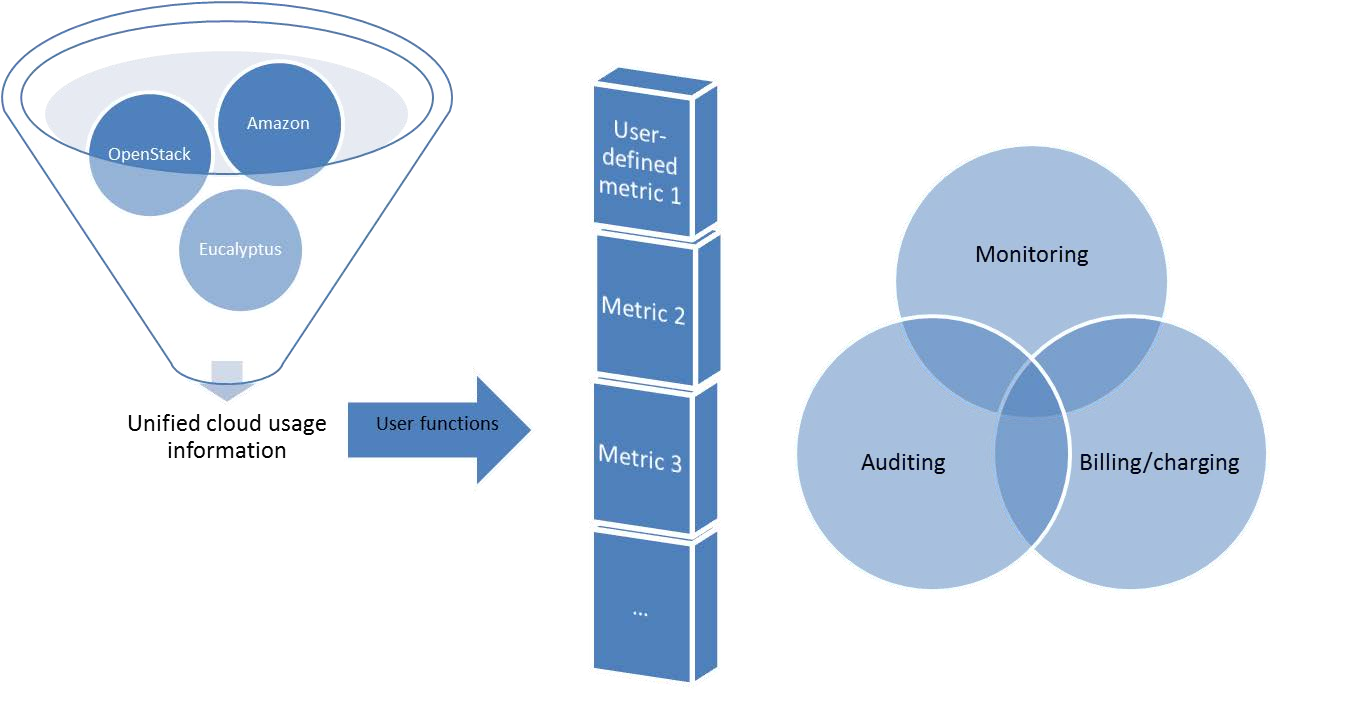
\includegraphics[width=1.0\textwidth]{images/Picture1.pdf} 
\end{center}
  \caption{Overview of CloudMetrics \hyungro{we need to redraw as
      color scheme is not so good for reproduction. what is original
      file? I hope this is pptx? Maybe this picture is not that
      important as contained already in architecture drawing? bu we do
    not see there auditing, monitoring, billing, as well as defining and
  adding new metrics. customization is something we missed in introduction.}}\label{F:fig1} 
\end{figure*} 



%CloudMetrics consists of four components: 1) a measuring tool of resource allocation  and 2) a CLI tool to define metrics and collect usage data 3) a visualization tool to provide graphical representative of the data and 4) Web Service APIs to support other applications e.g. scheduling and dynamic provisioning. We have the log parser named by fg-log-parser which reads and examines log messages of IaaS platforms (e.g. Eucalyptus, OpenStack) to collect metrics and stores the metrics into a database using a global object i.e. JSON converted from a python dictionary data type. fg-metrics takes the role of analyzing usage data and generating results in a image file or a csv file. We assume every measured data is stored in the database from five different resources (Foxtrot, Hotel, India, Sierra, Alamo) to support more than 400 projects and 3200 members as of 2014. Our new development of federation management, CloudMesh, uses the REST APIs to deliver accounting features on its command-line interfaces and web services~\cite{cloudmesh14}.

\subsection{Component}

Cloud Metrics consists of four components as described in Figure~\ref{F:fig7}: 1) Metric Collector: a measuring tool of resource allocation and 2) Metric Shell: a CLI tool to define metrics and collect usage data 3) Metric Portal and Report: a visualization tool to provide graphical representative of the data and 4) Web Service APIs to support other applications e.g. scheduling and dynamic provisioning. We have the log parser named by fg-log-parser which reads and examines log messages of IaaS platforms (e.g. Eucalyptus, OpenStack) to collect metrics and stores the metrics into a database using a global object i.e. JSON converted from a python dictionary data type. fg-metrics takes the role of analyzing usage data and generating results in a image file or a csv file. We assume every measured data is stored in the database from five different resources (Foxtrot, Hotel, India, Sierra, Alamo) to support more than 400 projects and 3200 members as of 2014. Our new development of federation management, CloudMesh, uses the REST APIs to deliver accounting features on its command-line interfaces and web services~\cite{las14cloudmeshmultiple}.

\begin{figure*}[htb] 
\begin{center}
 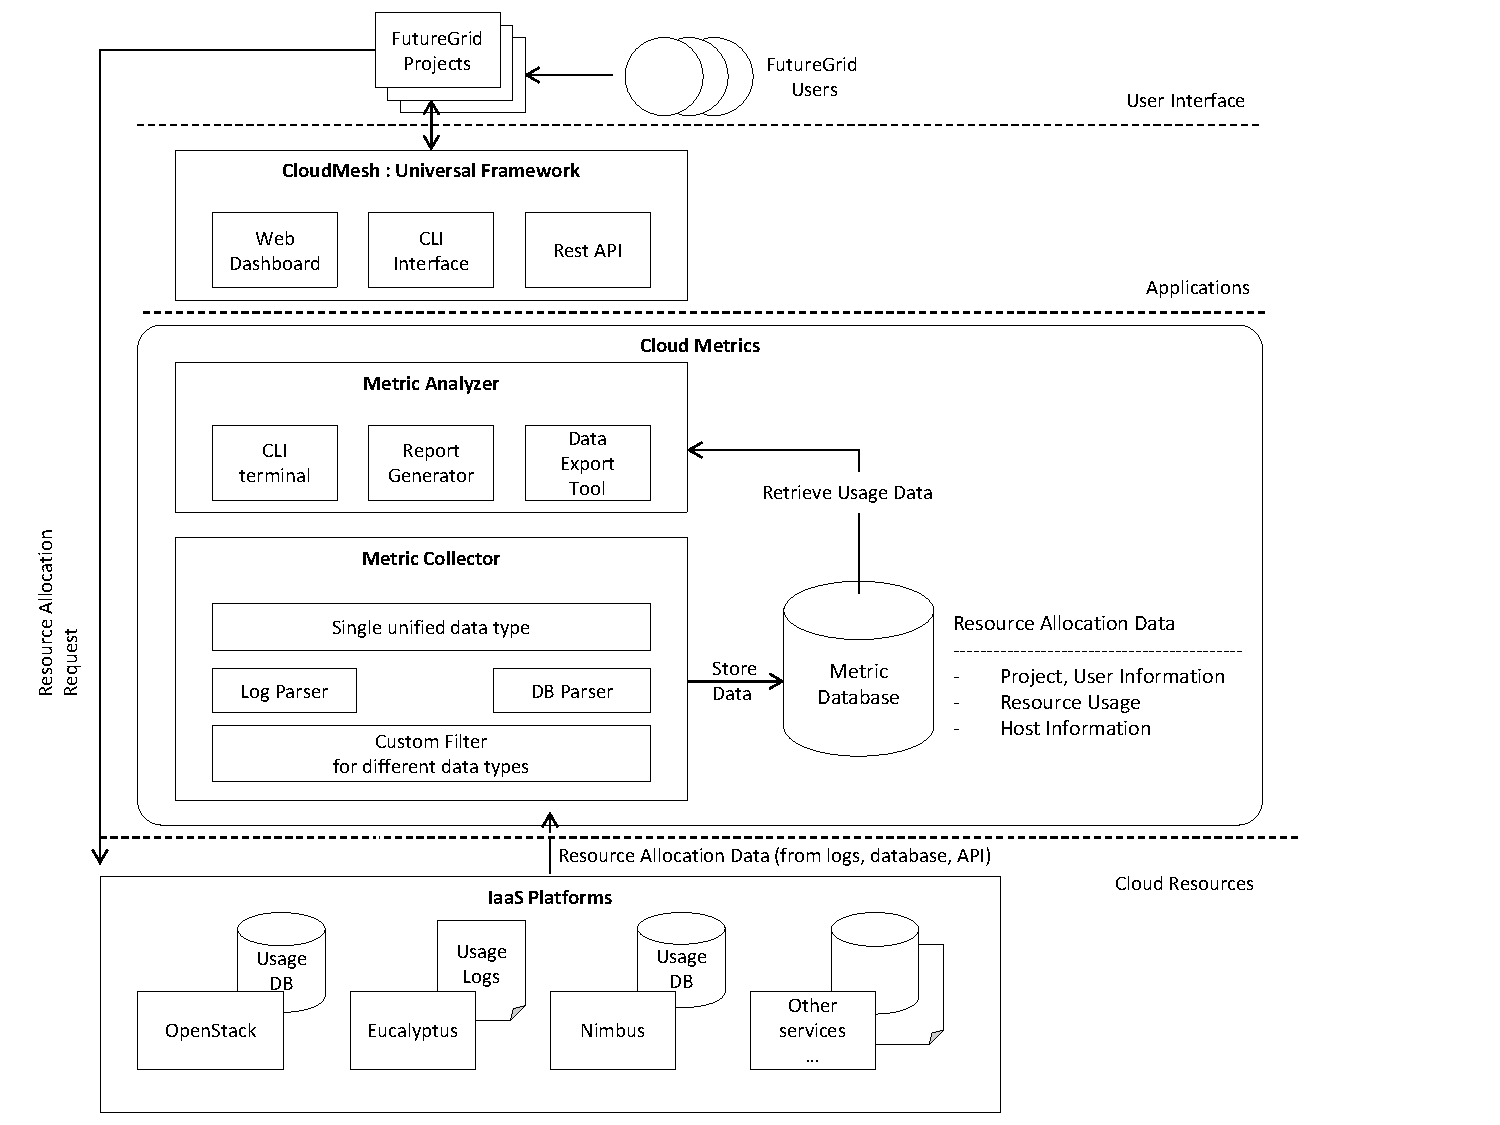
\includegraphics[width=1.0\textwidth]{images/system_overview.pdf} 
\end{center}
  \caption{Overview of Cloud Metrics \hyungro{we need to redraw, can
      this be dne in ppt or omni graffel}}\label{F:fig7} 
\end{figure*} 


\subsection{Metric Collector}

The Metric Collector is the sensor for collecting usage data allocated from IaaS cloud platforms such as Eucalyptus, Nimbus, and OpenStack including HPC from TORQUE. The collecor enables real-time monitoring and statistics by fg-metric-converter and fg-log-parser which are executable python scripts on Linux/Unix shell. fg-metric-converter (aggregator) imports usage data from a certain database such as MySQL or sqlite3 to the unified database. Account information such as a user name and a project associated with are also imported to the main database so the overall usage data can be viewed for vm instances and jobs launched on FutureGrid resources. OpenStack and Nimbus are measured by fg-metric-converter and Eucalyptus is measured by fg-log-parser. On the management nodes of cloud platforms, usage data can be captured in a format of logs or databases at a regular interval. Eucalyptus provides detailed information in a log file (cc.logs) which is generated by the compute controller (CC), about the number of launched instances, vCPUs, memories, disks and runtime. fg-log-parser collects these data from logs of the compute controlloer of eucalyptus. These two scripts are about to collect information of resource allocation from virtual machine instances (VMs). To get the information from Eucalyptus and OpenStack, basic templates are used to parse log messages using our pre-defined regular expressions. These are critical for that what type of log events will be collected and how it will be parsed without parsing errors and missing events. We have examined log messages of Eucalyptus and OpenStack and created templates for their instance information i.e. print\_ccInstance() function and nova.compute.resource\_tracker in a debug logging mode. Our custom templates for these IaaS platforms parse the events of the logs in a periodic basis or a real-time. There are basic metrics such as userid, instanceid, time values of a vm instance, a number of virtual cpu cores, disks, and a size of memories.

\subsection{Metric Analysis}

\begin{figure}[htb] 
  \centering 
    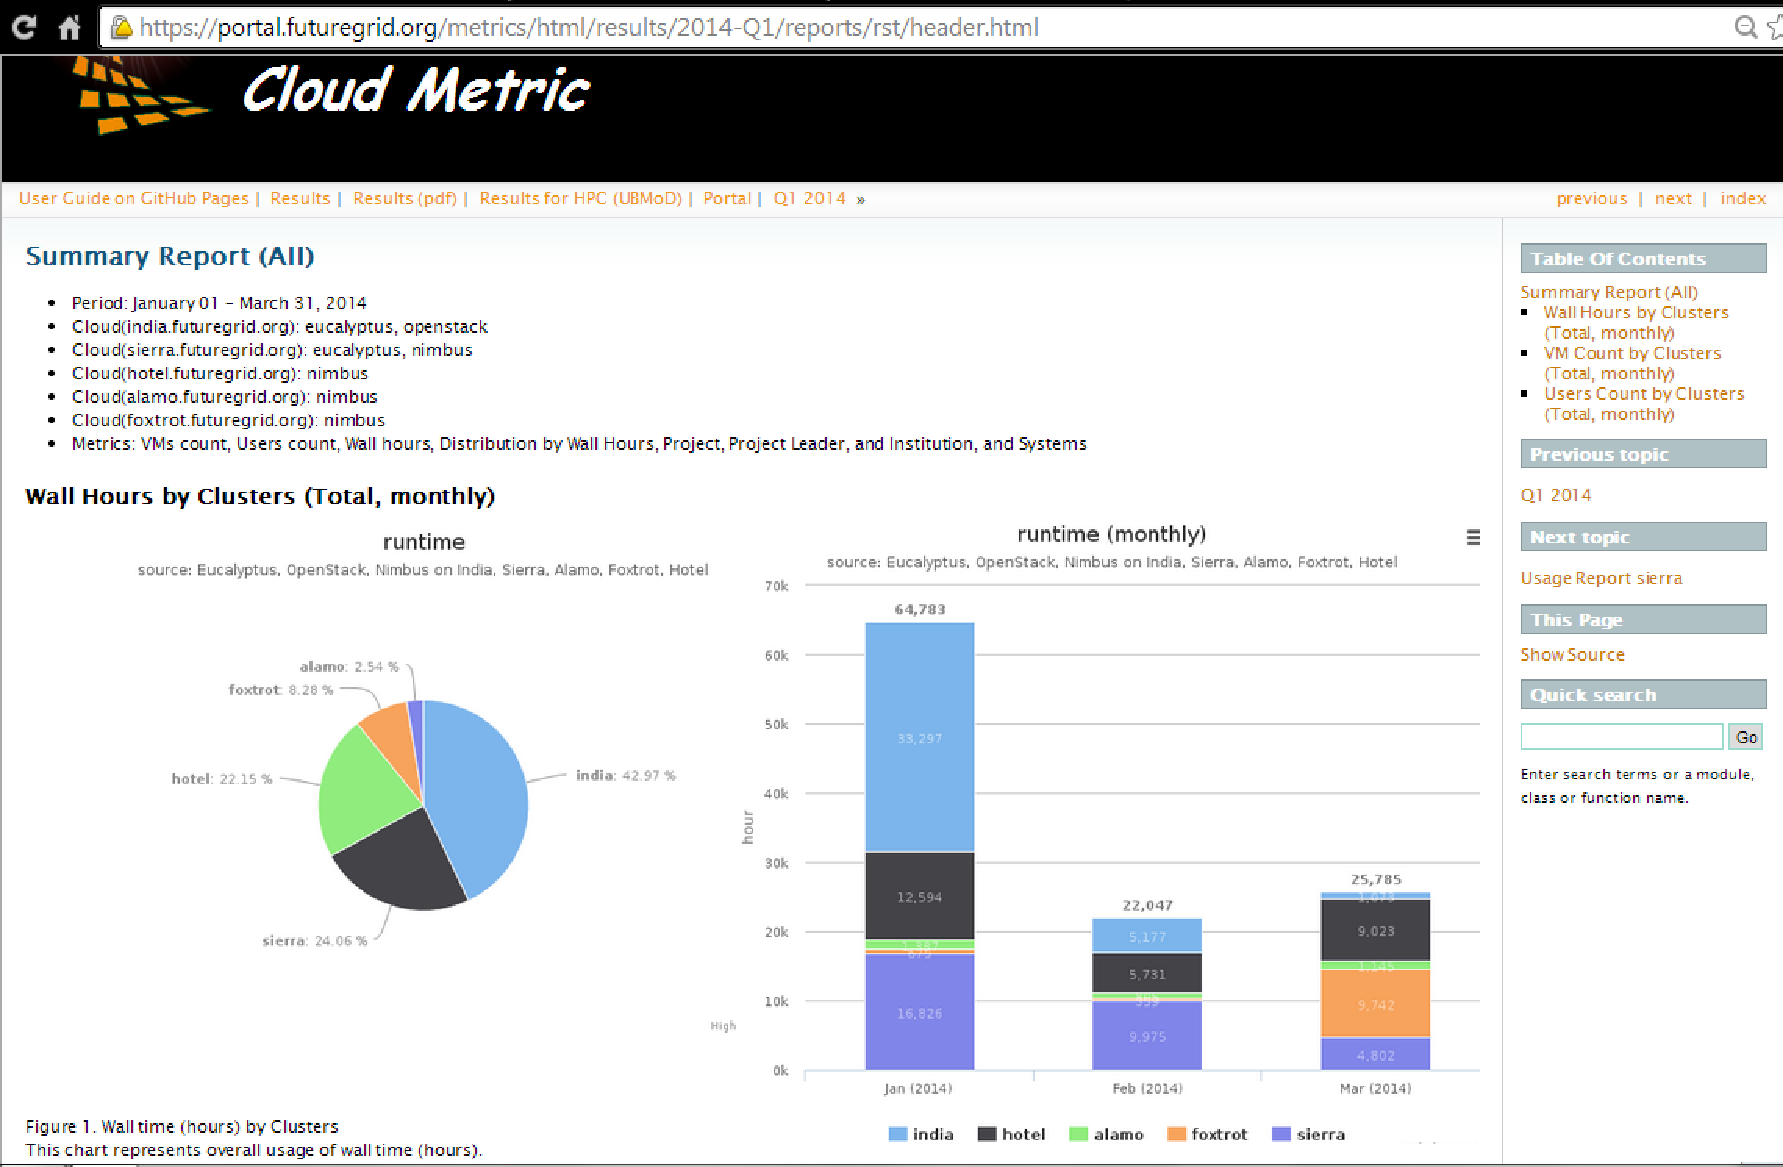
\includegraphics[width=1.0\columnwidth]{images/metrics-portal.pdf} 
  \caption{Cloud Metrics Portal: pie chart and stacked bar chart represent monthly usage of FutureGrid resources. Summary of regional clusters and different IaaS cloud platforms are displayed with various charts and different terms including monthly, quarterly and yearly.}\label{F:fig8} 
\end{figure} 

\begin{figure}[htb] 
  \centering 
    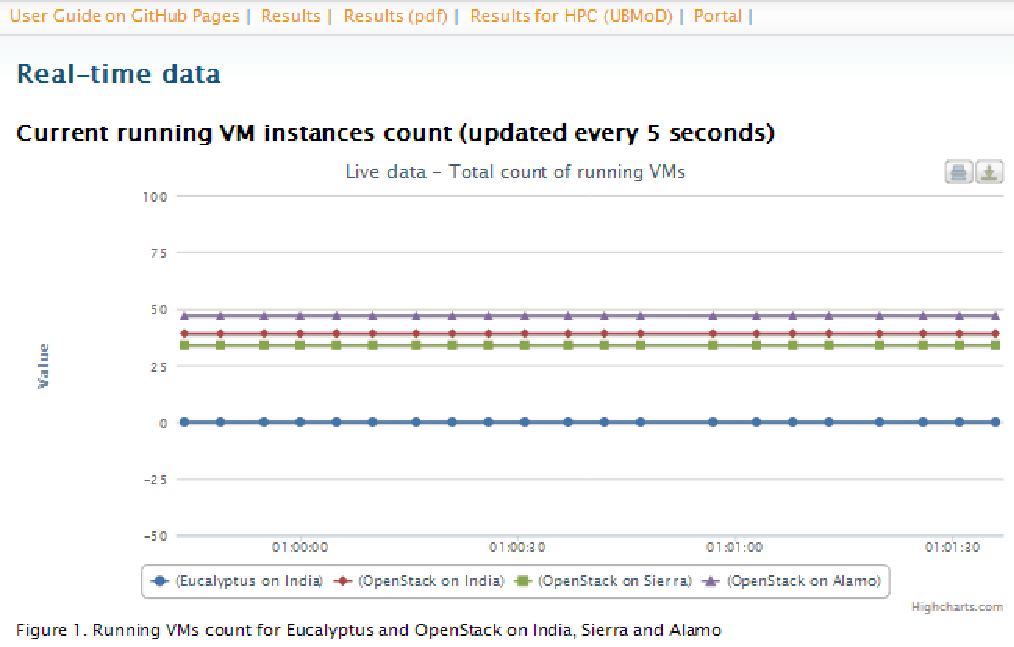
\includegraphics[width=1.0\columnwidth]{images/metrics-portal-realtime.pdf} 
  \caption{Real-time usage report on Cloud Metrics Portal: In every 5 seconds, the line chart is updated with the number of working virtual machine instances.}\label{F:fig9} 
\end{figure} 

In FutureGrid~\cite{las2010gce,las12fg-bookchapter}, users have a unique account id along with a project id across 8 different resources (Alamo, Bravo, Delta, Foxtrot, Hotel, India, Sierra, and Xray). The Metric analysis tool named by fg-metrics searches usage information across distributed resouces and services with their unique id and provides results with search options. For example, a user can specify the options using basic commands such as 'set nodename india' and 'set date -M 05 -Y 2012' to get usage information of India resource on May 2012. In addition, it supports different output types to help understanding statistics. Comma-separated values (CSV) files and graphical representation tools such as Google Chart API, Highcharts, D3.js, and jQuery Sparkline are used to generate results in image files (e.g. png, gif, and jpg).

\subsection{Results and Statistical Analysis} \label{S:result}

Based on the observation on FutureGrid, there is a different pattern between a research project and class work when they acquire cloud resources. Resource allocation of academic coursework shows time dependent request patterns. It shows a surge when there is a class, a lab session, and a project. For example, the undergraduate course for Distributed Systems at Indiana University introduced IaaS in the class and used the IaaS platform for a class project. Figure~\ref{F:fig2} shows a spike in the class and variability until the project due. A research project, on the contrary, requests VM instances in a steady usage. The Next Generation Sequencing (NGS) in the cloud project on FutureGrid shows relatively consistent resource allocation requested in Figure~\ref{F:fig3}. With a certain period of time, vm instances of this project have been launched without unplanned spike requests. These two examples show different patterns for deploying resources but both cases have a factor to predict loads. The class schedule and the monitoring data for applications can be used to measure the amount of resources and identify incoming requests. In paid cloud platforms such as AWS, GCE, and Azure, understanding these patterns is important to bring cost effectiveness over on-demand allocation. For example, Amazon EC2 Reserved Instances and Azure pre-pay plans may help reduce usage costs for periodic and planned workloads. These service plans simply provide discounts with an upfront payment. As long as a class and a project go as planned, cost saving chances are increased.

\begin{table}[htb]
  \caption{New accounts in FutureGrid}\label{T:tab00}
  \begin{tabular}{l|c|c}
   Year & Users & Projects \\
   \hline
   2011 & 637 & 100 \\
   2012 & 900 & 114 \\
   2013 & 614 & 103 \\
 \end{tabular}\\
 \end{table}

 \begin{table}[htb]
   \caption{Active Users in Cloud, HPC or Both}\label{T:tab000}
   \begin{tabular}{l|c|c|c}
     Year & Cloud & HPC & Both \\
     \hline
     2011 & 134 (123) & 154 (120) & 33 (26) \\
     2012 & 195 (130) & 164 (122) & 183 (144) \\
     2013 & 235 (140) & 200 (133) & 70 (38) \\
   \end{tabular}\\
   $^*$ New users shown in parenthesis
 \end{table}

 In average, FutureGrid accepted more than 100 projects every year, and around 60 to 90 members participated in each project. In table~\ref{T:tab000}, we noticed that more user were getting used both Cloud and HPC over the years instead of only using either Cloud or HPC. It implies that Cloud and HPC together can be beneficial to users.


\begin{figure}[htb] 
  \centering 
    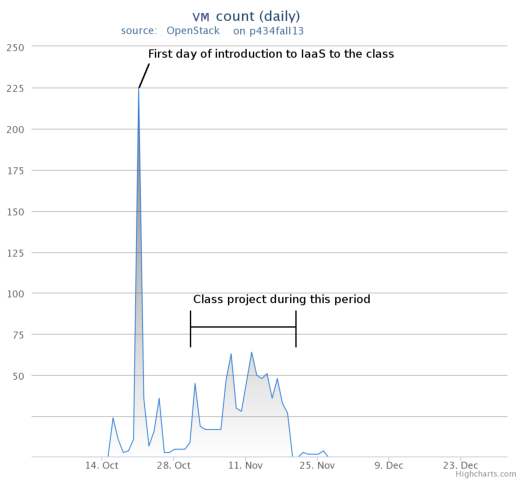
\includegraphics[width=1.0\columnwidth]{images/fig1.pdf} 
  \caption{IaaS Usage data for the Distributed System class at Indiana University*}\label{F:fig2} 
\end{figure} 


% * Based on the class schedule and metrics. Class schedule is here: http://salsahpc.indiana.edu/csci-p434-fall-2013/
% Metrics is here: http://129.79.49.94/accounting/reports/custom/p434fall13/FGResourceReport.pdf

\begin{figure}[htb] 
  \centering 
    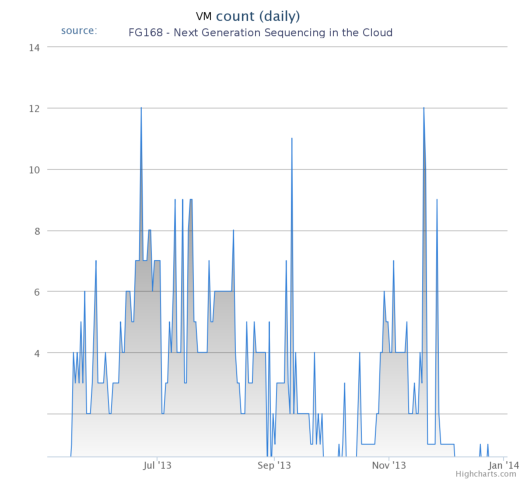
\includegraphics[width=1.0\columnwidth]{images/fig2.pdf} 
  \caption{VM count for Next Generation Sequencing (NGS) in the cloud project}\label{F:fig3} 
\end{figure} 

With the Gantt chart in Figure~\ref{F:fig4}, allocation activities are viewed for all virtual instances launched for the class. At the beginning of the class, the gaps between the start and completed dates of the vm instances are small but a large number of instances are initiated. Once the class is became operative, the runtime of vm instances is getting longer and a less number of instances are requested compared to the beginning. This observation tells us that academic projects require training sessions at the beginning of a project to get familiar with using infrastructure and to prepare environments by installing software and datasets.

\begin{figure}[htb] 
  \centering 
    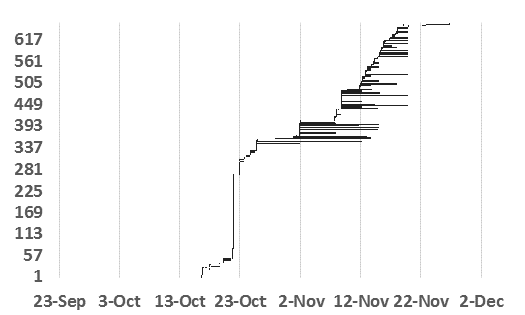
\includegraphics[width=1.0\columnwidth]{images/fig3.pdf} 
  \caption{Timeline for VM walltime}\label{F:fig4} 
\end{figure} 

Other observation is a resource usage for administrative purposes. Figure~\ref{F:fig5} describes that instructors consumed a large number of vCPU cores before class starts and small tests just before class projects. It indicates that the preparation of courses require extensive load testing on cloud resources to estimate compute capacity needed for applications.

\begin{figure}[htb] 
  \centering 
    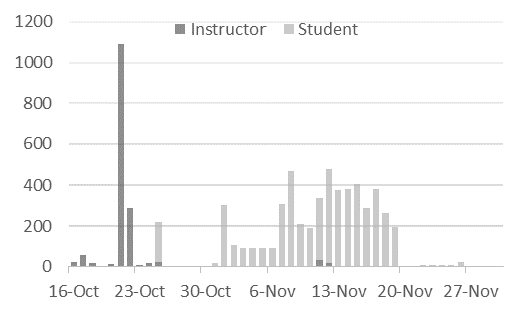
\includegraphics[width=1.0\columnwidth]{images/fig4.pdf} 
  \caption{Usage between instructors and students for vCPU cores}\label{F:fig5} 
\end{figure} 

During the semester, 25 hosts, 216 vCPUs and 600GB memories were reserved for the class since it required large virtual instances. In Figure~\ref{F:fig6} shows that the dedicated resources were being underutilized most time although the high volume requests had been made a few times including 273\% overutilization on October 21th for testing and preparing.
  
\begin{figure}[htb] 
  \centering 
    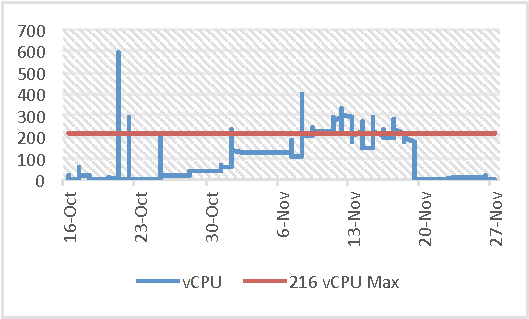
\includegraphics[width=1.0\columnwidth]{images/fig5.pdf} 
  \caption{vCPU Utilization (approximation per hour)}\label{F:fig6} 
\end{figure} 

High Performance Computing (HPC) has been used to support parallel data processing of Big Data. With Figure~\ref{F:bigdata}, we can see big data projects have also requested HPC and other services to work on their projects. HPC is the most requested services to whom also requested big data services and IaaS cloud platforms are also requested many times followed by HPC. It explains that platform hybrid implementations are one of today's trends for big data scientists and researchers. Regarding IaaS cloud platforms, there are three difference choices between OpenStack, Eucalyptus, and Nimbus on the FutureGrid test-bed. One observation from Figure~\ref{F:bigdata} is that OpenStack has taken Eucalyptus share since 2011 and became the most popular IaaS platform last year (2013). According to the recent report from RightScale~\cite{rightscalereport13}, cloud competition is heating up not only in public cloud including Amazon Web Services (AWS) and Google Compute Engine (GCE), but also in private cloud. The report shows that OpenStack is the most popular cloud environment for private cloud users so the changes in Figure~\ref{F:bigdata} is understandable in terms of finding cloud alternatives.

\begin{figure}[htb]
  \centering
    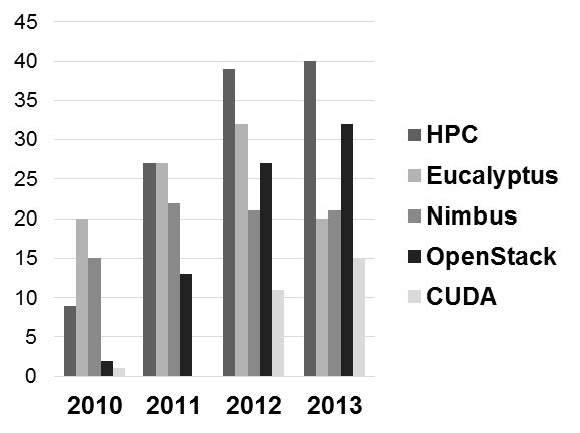
\includegraphics[width=1.0\columnwidth]{images/bigdata.pdf} 
  \caption{Service changes for along with Big Data between 2010 and 2013}\label{F:bigdata} 
\end{figure} 

In HPC, 64 and 128 CPU cores per job are most popular job sizes in FutureGrid HPC in 2013 (See Figure~\ref{F:bigdatainhpc}). 24\% and 14\% of total wall time are for 64 and 128 cpu jobs. An extra large jobs (i.e. 512 CPU cores) has been intensively used in the last year. Compared to the previous year 2012, the request has been increased about 350\%. In early stage of FutureGrid between 2010 and 2011, tiny CPU jobs have been requested many times but in 2013, two thirds jobs are using more than 64 CPU cores.

\begin{figure}[htb]
  \centering
    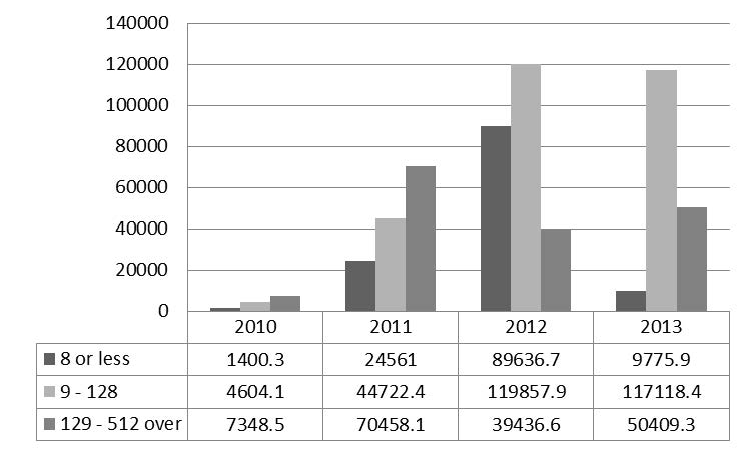
\includegraphics[width=1.0\columnwidth]{images/bigdatainhpc.pdf} 
  \caption{Annual Wall Time Changes for Job Size in HPC between 2010 and 2013}\label{F:bigdatainhpc} 
\end{figure} 

\begin{comment}

\subsection{Pricing Comparison}

Comparing pricing of the cloud is complicated and may lead to false analogy because each cloud provider offers various services with different performance. The pricing comparison, however, is important when people start to consider adopting cloud services among a lot of selections from different providers. In the comparison, important criteria are revealed through its pricing table. For example, there are a range of service offered, a size of available systems, costs, discounts and benefits such as technical support, and development tools. Amazon AWS, Windows Azure, Google Compute Engine (GCE), HP Cloud, IBM and Rackspace are compared. Pricing is scenario based. It can't be simply compared with numbers. GCE looks cheaper than other competitors, but others have several options to reduce cost. For example, a pay-ahead model provides a discount for same instances, and a spot instance also provides a way of saving entire cost for task intensive workloads in a small amount of time. In Table~\ref{T:tab0}, different price tags for virtual machine instances are described. With the comparison of the smallest vm instance which is 1 virtual core, 600-768MB memory and no storage option, we can see most IaaS service providers have similar pricing charts.

\begin{table}[htb]

%\caption{Pricing chart for instances from AWS, GCE, and Azure \newline * China (Beijing) region will be available in early 2014, and GovCloud region is also included.}\label{T:tab0}

 
\caption{Pricing chart for instances from AWS, GCE, and Azure}\label{T:tab0}
%\begin{footnotesize}
%\begin{tabular}{l|p{2.5cm}|l|p{2cm}}
 %    &  \shortstack{Billing\\ granularity} &   Price & \shortstack{Price\\ Variation} \\
 % \hline
%AWS &   By hour & \$0.02 &      \shortstack{10 regions*,\\ 6 platforms} \\
%GCE &   By minute$^1$ &       \$0.019  &      \shortstack{2 regions\\ (US, Europe)} \\
%Azure & By minute$^2$ & \$0.02 &    \shortstack{6 regions,\\ 5 platforms} \\
%\end{tabular}\\
%$^1$ with a minimum of 10 minutes\\
%$^2$ with a no minimum and free of charge for less than 5 minutes
\end{table}

\subsubsection{Example of Pricing Comparison}

We tried to apply each pricing model; Amazon AWS, Google Compute Engine, Microsoft Azure; to the usage data of the class (P434 distributed systems at Indiana University), to compare cost estimate of cloud resources. Google Compute Engine is the least expensive and 16\% lower than Amazon AWS. It is mostly because of that Google has 10\% discount pricing chart compared to AWS. We observed that a minute basis charge is only 3.3\% less expensive for this class. Some restrictions and offers such as Google's 10-minute minimum charge and Azure's less 5-minute free of charge are relatively small amount of a discount or an extra charge. Google's 10-minute minimum charge asks 0.18\% extra charge to the class, Azure provides 0.05\% discount through their less 5-minute free of charge. Amazon only has an hourly based pricing model, while Google Compute Engine and Windows Azure offer a minute basis charge for use of virtual machine instances. Three types of instances (small/medium/large) had been used for its coursework and projects and usage of virtual machine instances was only calculated without network and storage usage. Table~\ref{T:tab1}, ~\ref{T:tab2} shows pricing comparison to the class.

\begin{table}[htb]
\caption{Usage data to the class}\label{T:tab1}
\begin{footnotesize}
\begin{tabular}{l|r|l|l|r|r}
\shortstack{Instance\\types} & \shortstack{Instan-\\ces} & \shortstack{Charge\\by hour} & \shortstack{Charge\\by min} & Google$^1$ & Azure$^2$ \\
  \hline
small & 165 & 37,140 & 29,622 & 29,875 &29,582 \\
medium & 6 & 16,080 & 15,891 & 15,891 & 15,891 \\
large & 490 & 649,860 & 629,969 & 631,047 & 629,667 \\
  \hline \hline
Total & 661 & 703,080 & 675,482 & 676,813 & 675,140 \\
\end{tabular}\\
$^1$ includes 10~min minimum charge\\
$^2$ includes 5~min free charge
\end{footnotesize}
\end{table}

%* Instance types are not same. Chosen by a similarity of vCPU and Memory
%** Captured by January, 2014

\begin{table}[htb]
\caption{Pricing comparison to the class}\label{T:tab2}
\begin{footnotesize}
\begin{tabular}{l|l|l|l|l|l|p{2cm}|}
Service & Cost & \multicolumn{3}{|c|}{Price per hour} \\
  & Estimate &  Small& Medium& Large \\
 \hline
AWS$^1$ & \$2,668.74  & \$0.06 & \$0.12 & \$0.24 \\
GCE$^2$ & \$2,231.54  & \$0.054 & \$0.104 & \$0.207 \\
Azure$^3$ & \$2,580.03  & \$0.06 & \$0.12 & \$0.24 \\ 
\end{tabular}
\\
\\
$^1$US East, Linux, charged 1 hour if runtime is <1 hour\\
$^2$US, Linux, charged 10 minutes if runtime is <10 minutes\\
$^3$Linux, charged by minute but free is <5 minutes\\
\end{footnotesize}
\end{table}

\end{comment}

%%%%%%%%%%%%%%%%%%%%%%%%%%%%%%%%%%%%%%%%%%%%%%%%%%%%%%%%%%%%%%%%%%%%%% 
\section{RELATED WORK}\label{S:related}
%%%%%%%%%%%%%%%%%%%%%%%%%%%%%%%%%%%%%%%%%%%%%%%%%%%%%%%%%%%%%%%%%%%%%% 


\task{This section will contain some relevant related work. We have
  included a small set of references that may be helpful to establish
  this section}

Nist~\cite{NIST2015}
Blueflood~\cite{BlueFloodDB}
CM-measurement facets for cloud performance~\cite{singh2011cm}
Online detection of utility cloud anomalies using metric distributions~\cite{wang2010online}
M4Cloud-Generic Application Level Monitoring for Resource-shared Cloud Environments.~\cite{mastelic2012m4cloud}
Design of a Dynamic Provisioning System for a Federated Cloud and Bare-metal Environment~\cite{vondesign}
\cite{CloudAuditingDataFederation}
\cite{viewing-keystone-cadf-notifications-with-ceilometer-and-rabbitmq}
\cite{GoogleCustomMetrics}
\cite{terencengai}
\cite{KevinFogarty}
\cite{SharonWagner}
\cite{MarcusSarmento}
\cite{awscloudwatch}
\cite{RobBoucher}
\cite{GregorBeslic}
\cite{aceto2013cloud}
\cite{HPHelionEucalyptus}
\cite{eucalyptusgithub}
\cite{ceilometer}
\cite{gcemonitoring}

\cite{securitymetrics}
\cite{securitymetrics-educause}

\subsection{Surveys and Taxonomies}
\begin{verbatim}
\cite{vineetha2012performance}
\cite{alhamazani2013overview}
\cite{fourkeys-for-monitoring}

\cite{aceto2012cloud}
\cite{clayman2010monitoring}
\cite{fatema2014survey}
\cite{paessler2012monitoring}
\cite{mohamaddiah2014survey}
\cite{brinkmann2013scalable}
\cite{gorbil2014principles}
\cite{ward2014observing}
\cite{danetwork}
\cite{petcu2014towards}
\cite{zhang2013survey}
\end{verbatim}

see what shava and w smith did check previous xsede conferences

rightscale


%%%%%%%%%%%%%%%%%%%%%%%%%%%%%%%%%%%%%%%%%%%%%%%%%%%%%%%%%%%%%%%%%%%%%%
\section{CONCLUSION}\label{S:conclusion}
%%%%%%%%%%%%%%%%%%%%%%%%%%%%%%%%%%%%%%%%%%%%%%%%%%%%%%%%%%%%%%%%%%%%%%


We hope this activity provides a way of understanding performance and resource utilization across system and application layers, especially on cloud resources. With the various requests of resource allocation on the cloud, project leaders and members encounter challenges with finding availability of virtual resources and handling this information. Cloud users in a pool of shared resources can suffer performance degradation by other users. Monitoring physical resources is not enough to mitigate this degradation in cyberinfrastructure. In this paper, Cloud Metrics offer several means to get information of resource utilization and performance. In addition, the classification of performance managements and case studies provide an inside visibility to help identify the issues easily and finding solutions regarding resource allocation on the cloud. To enhance performance of systems and get powerful machines, understanding resource allocation of virtual resources is needed to avoid under performing systems and applications.

\task{We can think about rerouting VM instances to ensure scalable services by avoiding crowded zone. This cloud shifting may support relaxed management regarding load balancing of the cloud systems. The other potential work is probably that we can provide an indicator of cost-efficient leasing on the cloud based on the correlation data measured by this activity. Cost of using cloud can be reduced in many ways, including finding inexpensive cloud service providers, and using parallel processing technique such as MapReduce. Measuring correlation between physical and virtual resources could mean that we can find a spot in which reliable performance is guaranteed and it would be one of the main techniques to provide cost-efficient cloud renting across all the resources.}

% scheduling

%In a sense of security, accounting is also able to provide some information for investigation of suspected security intrusions not only providing resource usage1 monitoring. Billing is another purpose of accounting.



% \begin{sidewaystable*}
% \caption{table 3}\label{T:tab3}
% 
% \begin{footnotesize}
% \begin{tabular}{|p{2cm}|p{2cm}|p{1.5cm}|p{1.5cm}|p{2cm}|p{1cm}|p{1.5cm}|p{2cm}|p{2cm}|p{2cm}|}
% \hline
% Provider & Charging & Cost 1vCPU/hour    & Cost 1GB/hour & OS & Max vCPU & Memory min - max &\# of instance types & Discount program & Free allowance\\
% \hline
% \hline
% Aws & hourly & \$0.04  & \$0.02  & Linux & 32 & 615MB - & 22 & spot instance;  & \$100 for educators and student\\
%     &              &         &         & Windows +14-56\%     &    & 244GB    &       & reserved instances & Grant for researcher, AWS educated grant program\\
%     &              &         &         & Asia + 25\%          &    &                 &       &                    & \\
% \hline
% Google Compute Engine & 10 minutes + & \$0.08  & \$0.01  & Linux (Debian; CentOS) & 16 & 600MB - & 1- & n/a & Google app reward programs\\
%  & every minute after that &  &  & (RHEL; SUSE premium operating systems) *** &  & 104GB & (4 high cpu + 4 high memory + 2 small + 5 standard) &  & \$1000 for educator\\
%  &  &  & Europe + 4.5\% - 27\%  &  &  &  &  &  & \$60;000 for research project\\
% \hline 
% IBM CloudLayer (by Softlayer) & monthly & \$0.50  & varies & Linux;  & 16 & 1GB  & Build your own cloud server offers customized options &  & one month trial for 1 vcpu + 1gb memory + 25 storage\\
% \hline
%  & hourly & to &  & Windows + \$0.05 to &  & -  &  &  & \\
%  &  & \$0.10  &  &               \$0.10 / hour &  & 64GB &  &  & \\
% \hline 
% HP cloud & hourly & \$0.02  & \$0.02  & Linux; Windows; SUSE & 16 & 1GB  & 11 (8 standard + 3 memory intensive) &  & \$300 free trial for 90 days (\$100 for each month)\\
%  &  &  &  & (windows: 10-200\% extra charge; &  & -  &  &  & \\
%  &  &  &  & SUSE: 4\% - 200\% extra charge) &  & 120GB &  &  & \\
% \hline 
% Microsoft Azure & Free first 5 minutes & \$0.05  & \$0.02 (approx.) & Linux;  & 8 & 768MB -  & 8 (A0-A7) & 6-Month; 12-month pre-pay membership & \$200 free trial of first month\\
%  &  &  & Windows is expensive 30-50\% more than linux & Windows + 30-50\%  &  & 56GB &  &  & \\
% \hline 
% Rackspace & minute &  & varies & Linux; Windows, (windows: 25\% extra charge) & 32 & 1GB - 120GB  & 9 & Volume discount (4\% to 20\% for spending over \$5;000 - \$ 10; 000 per month; 8\% for \$10;001 - 30;000; 12\% for \$30;001 - \$50;000) Commitment discount (4\% to 40\%) Prepayment discount with commitment (7\% to 55\%)& \$300 developer discount (\$50 each for six months)\\
% \hline
% \end{tabular}
% \end{footnotesize}
% \end{sidewaystable*}
% 
% 
% Provider      Charging        Cost
% 1 vCPU /hour  Cost
% 1 GB
% /hour OS      Max vCPU        Memory min - max        \# of instance types    Discount program        Free allowance
% Aws
%       hourly  \$0.04
%       $0.01927        Linux
% Windows +14-56% 
% Asia + 25%    32      615MB -
% 244GB 22      spot instance, 
% reserved instances    $100 for educator's student
% Grant for researcher
% AWS educated grant program
% Google Compute Engine 10 minutes +
% every minute after that       $0.0788
%       $0.006636
% 
% Europe + 4.5% - 27%   Linux (Debian, CentOS)
% (RHEL, SUSE premium operating systems) ***    16      600MB -
% 104GB 15
% (4 high cpu + 4 high memory + 2 small + 5 standard)   n/a     Google app reward programs
% $1000 for educator
% $60,000 for research project
% IBM CloudLayer (by Softlayer) monthly
% hourly        $0.5
% to
% $0.10 varies  Linux, 
% Windows + $0.05 to
%               $0.10 / hour    16      1GB 
% – 
% 64GB  Build your own cloud server offers customized options           one month trial for 1 vcpu + 1gb memory + 25 storage
% HP cloud      hourly  $0.015  $0.015  Linux, Windows, SUSE
% (windows: 10-200% extra charge,
% SUSE: 4% - 200% extra charge) 16      1GB 
% – 
% 120GB 11 (8 standard + 3 memory intensive)            $300 free trial for 90 days ($100 for each month)
% Microsoft Azure       Free first 5 minutes
%       $ 0.05  $0.02 (approx.)
% Windows is expensive 30-50% more than linux   Linux, 
% Windows + 30-50%      8       768MB – 
% 56GB  8 (A0-A7)       6-Month, 12-month pre-pay membership    $200 free trial of first month
% Rackspace     minute          varies  Linux, Windows
% (windows: 25% extra charge)   32      1GB – 
% 120GB 9       Volume discount (4% to 20% for spending over $5,000 - $ 10, 000 per month, 8% for $10,001 - 30,000, 12% for $30,001 - $50,000)
% Commitment discount (4% to 40%)
% Prepayment discount with commitment (7% to 55%)       $300 developer discount ($50 each for six months)



%%%%%%%%%%%%%%%%%%%%%%%%%%%%%%%%%%%%%%%%%%%%%%%%%%%%%%%%%%%%%%%%%%%%%% 
% Acknowledgment 
%%%%%%%%%%%%%%%%%%%%%%%%%%%%%%%%%%%%%%%%%%%%%%%%%%%%%%%%%%%%%%%%%%%%%% 
  
\section{ACKNOWLEDGEMENT} 
 
This material based upon work is partially supported in part by the National Science Foundation under Grant No. 1445806, 1445806, and 0910812.

%\clearpage 

\begin{scriptsize} 
\bibliographystyle{IEEEtranS} 
%\bibliographystyle{abbrv} 
\bibliography{% 
metric-new,%
bib/vonLaszewski-jabref,% 
bib/cyberaide-metric,%
bib/cyberaide-cloud,%
metric-new}
%bib/image-refs,% 
\end{scriptsize}
   
%bib/python,% 
%tas.bib%
 
\end{document} 
 

